% Created by tikzDevice version 0.12
% !TEX encoding = UTF-8 Unicode
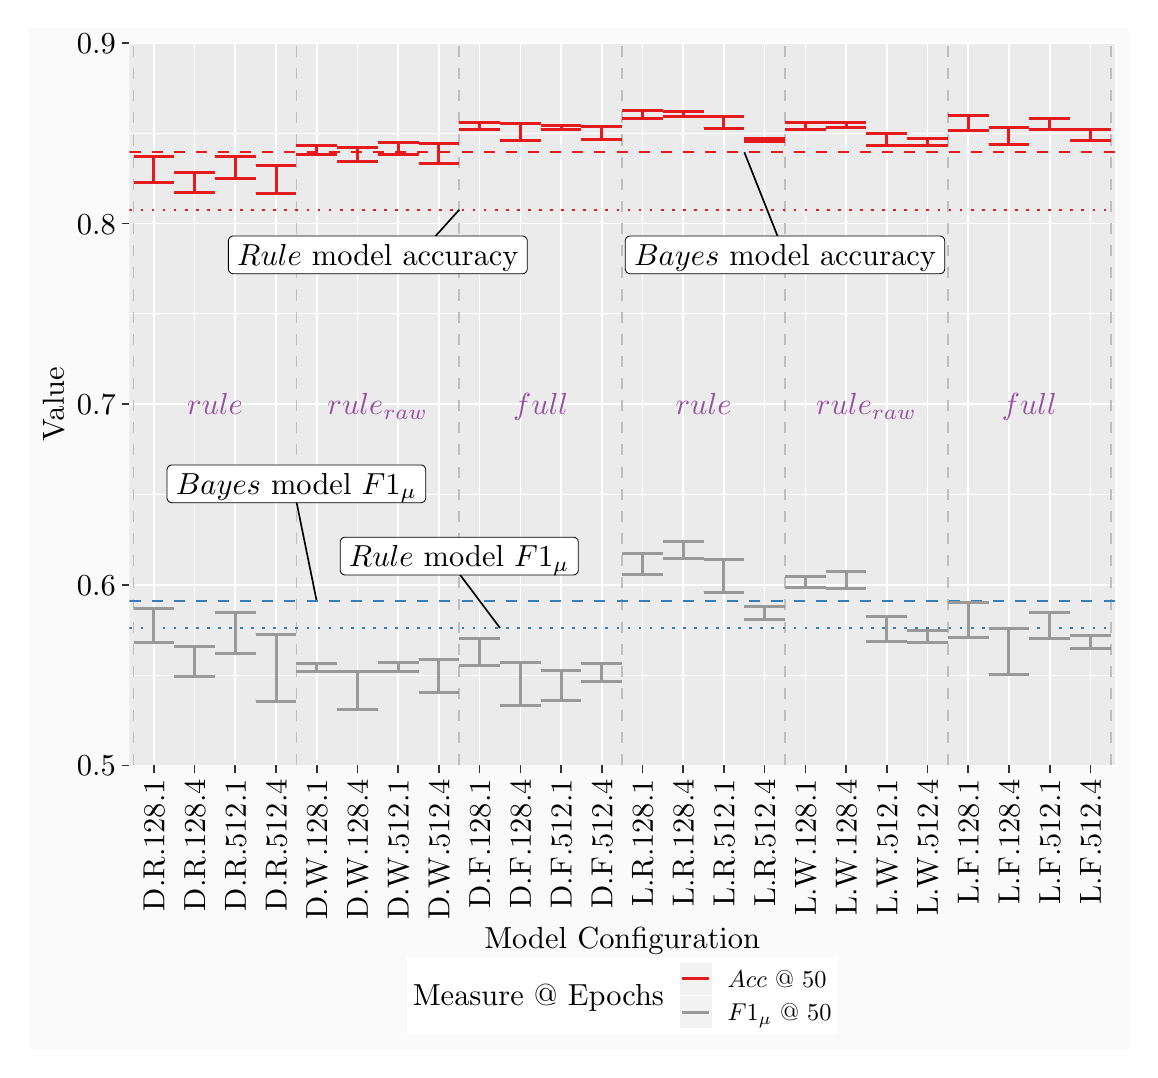
\begin{tikzpicture}[x=1pt,y=1pt]
\definecolor{fillColor}{RGB}{255,255,255}
\path[use as bounding box,fill=fillColor,fill opacity=0.00] (0,0) rectangle (398.34,369.26);
\begin{scope}
\path[clip] (  0.00,  0.00) rectangle (398.34,369.26);
\definecolor{drawColor}{RGB}{255,255,255}
\definecolor{fillColor}{gray}{0.98}

\path[draw=drawColor,line width= 0.6pt,line join=round,line cap=round,fill=fillColor] (  0.00,  0.00) rectangle (398.34,369.26);
\end{scope}
\begin{scope}
\path[clip] ( 36.77,102.67) rectangle (392.84,363.76);
\definecolor{fillColor}{gray}{0.92}

\path[fill=fillColor] ( 36.77,102.67) rectangle (392.84,363.76);
\definecolor{drawColor}{RGB}{255,255,255}

\path[draw=drawColor,line width= 0.3pt,line join=round] ( 36.77,135.31) --
	(392.84,135.31);

\path[draw=drawColor,line width= 0.3pt,line join=round] ( 36.77,200.58) --
	(392.84,200.58);

\path[draw=drawColor,line width= 0.3pt,line join=round] ( 36.77,265.85) --
	(392.84,265.85);

\path[draw=drawColor,line width= 0.3pt,line join=round] ( 36.77,331.12) --
	(392.84,331.12);

\path[draw=drawColor,line width= 0.6pt,line join=round] ( 36.77,102.67) --
	(392.84,102.67);

\path[draw=drawColor,line width= 0.6pt,line join=round] ( 36.77,167.94) --
	(392.84,167.94);

\path[draw=drawColor,line width= 0.6pt,line join=round] ( 36.77,233.22) --
	(392.84,233.22);

\path[draw=drawColor,line width= 0.6pt,line join=round] ( 36.77,298.49) --
	(392.84,298.49);

\path[draw=drawColor,line width= 0.6pt,line join=round] ( 36.77,363.76) --
	(392.84,363.76);

\path[draw=drawColor,line width= 0.6pt,line join=round] ( 45.60,102.67) --
	( 45.60,363.76);

\path[draw=drawColor,line width= 0.6pt,line join=round] ( 60.31,102.67) --
	( 60.31,363.76);

\path[draw=drawColor,line width= 0.6pt,line join=round] ( 75.03,102.67) --
	( 75.03,363.76);

\path[draw=drawColor,line width= 0.6pt,line join=round] ( 89.74,102.67) --
	( 89.74,363.76);

\path[draw=drawColor,line width= 0.6pt,line join=round] (104.45,102.67) --
	(104.45,363.76);

\path[draw=drawColor,line width= 0.6pt,line join=round] (119.17,102.67) --
	(119.17,363.76);

\path[draw=drawColor,line width= 0.6pt,line join=round] (133.88,102.67) --
	(133.88,363.76);

\path[draw=drawColor,line width= 0.6pt,line join=round] (148.59,102.67) --
	(148.59,363.76);

\path[draw=drawColor,line width= 0.6pt,line join=round] (163.31,102.67) --
	(163.31,363.76);

\path[draw=drawColor,line width= 0.6pt,line join=round] (178.02,102.67) --
	(178.02,363.76);

\path[draw=drawColor,line width= 0.6pt,line join=round] (192.74,102.67) --
	(192.74,363.76);

\path[draw=drawColor,line width= 0.6pt,line join=round] (207.45,102.67) --
	(207.45,363.76);

\path[draw=drawColor,line width= 0.6pt,line join=round] (222.16,102.67) --
	(222.16,363.76);

\path[draw=drawColor,line width= 0.6pt,line join=round] (236.88,102.67) --
	(236.88,363.76);

\path[draw=drawColor,line width= 0.6pt,line join=round] (251.59,102.67) --
	(251.59,363.76);

\path[draw=drawColor,line width= 0.6pt,line join=round] (266.30,102.67) --
	(266.30,363.76);

\path[draw=drawColor,line width= 0.6pt,line join=round] (281.02,102.67) --
	(281.02,363.76);

\path[draw=drawColor,line width= 0.6pt,line join=round] (295.73,102.67) --
	(295.73,363.76);

\path[draw=drawColor,line width= 0.6pt,line join=round] (310.44,102.67) --
	(310.44,363.76);

\path[draw=drawColor,line width= 0.6pt,line join=round] (325.16,102.67) --
	(325.16,363.76);

\path[draw=drawColor,line width= 0.6pt,line join=round] (339.87,102.67) --
	(339.87,363.76);

\path[draw=drawColor,line width= 0.6pt,line join=round] (354.58,102.67) --
	(354.58,363.76);

\path[draw=drawColor,line width= 0.6pt,line join=round] (369.30,102.67) --
	(369.30,363.76);

\path[draw=drawColor,line width= 0.6pt,line join=round] (384.01,102.67) --
	(384.01,363.76);
\definecolor{drawColor}{RGB}{190,190,190}

\path[draw=drawColor,line width= 0.6pt,dash pattern=on 4pt off 4pt ,line join=round] ( 38.24,102.67) -- ( 38.24,363.76);

\path[draw=drawColor,line width= 0.6pt,dash pattern=on 4pt off 4pt ,line join=round] ( 97.10,102.67) -- ( 97.10,363.76);

\path[draw=drawColor,line width= 0.6pt,dash pattern=on 4pt off 4pt ,line join=round] (155.95,102.67) -- (155.95,363.76);

\path[draw=drawColor,line width= 0.6pt,dash pattern=on 4pt off 4pt ,line join=round] (214.81,102.67) -- (214.81,363.76);

\path[draw=drawColor,line width= 0.6pt,dash pattern=on 4pt off 4pt ,line join=round] (273.66,102.67) -- (273.66,363.76);

\path[draw=drawColor,line width= 0.6pt,dash pattern=on 4pt off 4pt ,line join=round] (332.51,102.67) -- (332.51,363.76);

\path[draw=drawColor,line width= 0.6pt,dash pattern=on 4pt off 4pt ,line join=round] (391.37,102.67) -- (391.37,363.76);
\definecolor{drawColor}{RGB}{152,78,163}

\node[text=drawColor,anchor=base,inner sep=0pt, outer sep=0pt, scale=  1.10] at ( 67.67,229.41) {\(rule\)};

\node[text=drawColor,anchor=base,inner sep=0pt, outer sep=0pt, scale=  1.10] at (126.52,229.41) {\(rule_{raw}\)};

\node[text=drawColor,anchor=base,inner sep=0pt, outer sep=0pt, scale=  1.10] at (185.38,229.41) {\(full\)};

\node[text=drawColor,anchor=base,inner sep=0pt, outer sep=0pt, scale=  1.10] at (244.23,229.41) {\(rule\)};

\node[text=drawColor,anchor=base,inner sep=0pt, outer sep=0pt, scale=  1.10] at (303.09,229.41) {\(rule_{raw}\)};

\node[text=drawColor,anchor=base,inner sep=0pt, outer sep=0pt, scale=  1.10] at (361.94,229.41) {\(full\)};
\definecolor{drawColor}{RGB}{0,0,0}

\path[draw=drawColor,line width= 0.6pt,line join=round] (141.24,287.16) --
	(155.95,303.47);

\path[draw=drawColor,line width= 0.6pt,line join=round] (258.95,324.27) --
	(273.66,287.16);

\path[draw=drawColor,line width= 0.6pt,line join=round] (155.95,171.94) --
	(170.66,152.36);

\path[draw=drawColor,line width= 0.6pt,line join=round] ( 97.10,198.05) --
	(104.45,161.99);
\definecolor{fillColor}{RGB}{255,255,255}

\path[draw=drawColor,line width= 0.3pt,line join=round,line cap=round,fill=fillColor] ( 52.17,197.61) --
	(142.02,197.61) --
	(141.95,197.61) --
	(142.24,197.62) --
	(142.53,197.68) --
	(142.80,197.78) --
	(143.05,197.93) --
	(143.28,198.11) --
	(143.47,198.33) --
	(143.62,198.57) --
	(143.74,198.84) --
	(143.81,199.12) --
	(143.83,199.41) --
	(143.83,199.41) --
	(143.83,209.43) --
	(143.83,209.43) --
	(143.81,209.72) --
	(143.74,210.00) --
	(143.62,210.27) --
	(143.47,210.51) --
	(143.28,210.73) --
	(143.05,210.91) --
	(142.80,211.06) --
	(142.53,211.16) --
	(142.24,211.22) --
	(142.02,211.23) --
	( 52.17,211.23) --
	( 52.39,211.22) --
	( 52.10,211.23) --
	( 51.81,211.20) --
	( 51.53,211.12) --
	( 51.27,210.99) --
	( 51.03,210.83) --
	( 50.82,210.62) --
	( 50.64,210.39) --
	( 50.51,210.13) --
	( 50.42,209.86) --
	( 50.37,209.57) --
	( 50.36,209.43) --
	( 50.36,199.41) --
	( 50.37,199.56) --
	( 50.37,199.27) --
	( 50.42,198.98) --
	( 50.51,198.71) --
	( 50.64,198.45) --
	( 50.82,198.22) --
	( 51.03,198.01) --
	( 51.27,197.85) --
	( 51.53,197.72) --
	( 51.81,197.64) --
	( 52.10,197.61) --
	cycle;
\end{scope}
\begin{scope}
\path[clip] ( 36.77,102.67) rectangle (392.84,363.76);
\definecolor{drawColor}{RGB}{0,0,0}

\node[text=drawColor,anchor=base,inner sep=0pt, outer sep=0pt, scale=  1.10] at ( 97.10,200.62) {\(Bayes\) model \(F1_\mu\)};
\definecolor{fillColor}{RGB}{255,255,255}

\path[draw=drawColor,line width= 0.3pt,line join=round,line cap=round,fill=fillColor] (114.75,171.50) --
	(197.15,171.50) --
	(197.08,171.50) --
	(197.37,171.51) --
	(197.66,171.57) --
	(197.93,171.67) --
	(198.18,171.82) --
	(198.41,172.00) --
	(198.60,172.22) --
	(198.75,172.47) --
	(198.87,172.73) --
	(198.94,173.02) --
	(198.96,173.31) --
	(198.96,173.31) --
	(198.96,183.32) --
	(198.96,183.32) --
	(198.94,183.61) --
	(198.87,183.89) --
	(198.75,184.16) --
	(198.60,184.40) --
	(198.41,184.62) --
	(198.18,184.80) --
	(197.93,184.95) --
	(197.66,185.05) --
	(197.37,185.11) --
	(197.15,185.12) --
	(114.75,185.12) --
	(114.97,185.11) --
	(114.68,185.12) --
	(114.39,185.09) --
	(114.11,185.01) --
	(113.84,184.88) --
	(113.61,184.72) --
	(113.40,184.52) --
	(113.22,184.28) --
	(113.09,184.03) --
	(112.99,183.75) --
	(112.95,183.46) --
	(112.94,183.32) --
	(112.94,173.31) --
	(112.95,173.45) --
	(112.95,173.16) --
	(112.99,172.87) --
	(113.09,172.60) --
	(113.22,172.34) --
	(113.40,172.11) --
	(113.61,171.91) --
	(113.84,171.74) --
	(114.11,171.62) --
	(114.39,171.54) --
	(114.68,171.50) --
	cycle;
\end{scope}
\begin{scope}
\path[clip] ( 36.77,102.67) rectangle (392.84,363.76);
\definecolor{drawColor}{RGB}{0,0,0}

\node[text=drawColor,anchor=base,inner sep=0pt, outer sep=0pt, scale=  1.10] at (155.95,174.51) {\(Rule\) model \(F1_\mu\)};
\definecolor{fillColor}{RGB}{255,255,255}

\path[draw=drawColor,line width= 0.3pt,line join=round,line cap=round,fill=fillColor] ( 74.34,280.34) --
	(178.71,280.34) --
	(178.64,280.34) --
	(178.93,280.36) --
	(179.21,280.41) --
	(179.48,280.52) --
	(179.73,280.66) --
	(179.96,280.85) --
	(180.15,281.06) --
	(180.31,281.31) --
	(180.42,281.58) --
	(180.49,281.86) --
	(180.51,282.15) --
	(180.51,282.15) --
	(180.51,292.16) --
	(180.51,292.16) --
	(180.49,292.45) --
	(180.42,292.73) --
	(180.31,293.00) --
	(180.15,293.25) --
	(179.96,293.47) --
	(179.73,293.65) --
	(179.48,293.79) --
	(179.21,293.90) --
	(178.93,293.96) --
	(178.71,293.97) --
	( 74.34,293.97) --
	( 74.56,293.96) --
	( 74.27,293.97) --
	( 73.98,293.93) --
	( 73.70,293.85) --
	( 73.44,293.73) --
	( 73.20,293.56) --
	( 72.99,293.36) --
	( 72.81,293.13) --
	( 72.68,292.87) --
	( 72.59,292.59) --
	( 72.54,292.31) --
	( 72.53,292.16) --
	( 72.53,282.15) --
	( 72.54,282.30) --
	( 72.54,282.00) --
	( 72.59,281.72) --
	( 72.68,281.44) --
	( 72.81,281.18) --
	( 72.99,280.95) --
	( 73.20,280.75) --
	( 73.44,280.59) --
	( 73.70,280.46) --
	( 73.98,280.38) --
	( 74.27,280.34) --
	cycle;
\end{scope}
\begin{scope}
\path[clip] ( 36.77,102.67) rectangle (392.84,363.76);
\definecolor{drawColor}{RGB}{0,0,0}

\node[text=drawColor,anchor=base,inner sep=0pt, outer sep=0pt, scale=  1.10] at (126.52,283.35) {\(Rule\) model accuracy};
\definecolor{fillColor}{RGB}{255,255,255}

\path[draw=drawColor,line width= 0.3pt,line join=round,line cap=round,fill=fillColor] (217.75,280.34) --
	(329.57,280.34) --
	(329.49,280.34) --
	(329.78,280.36) --
	(330.07,280.41) --
	(330.34,280.52) --
	(330.59,280.66) --
	(330.82,280.85) --
	(331.01,281.06) --
	(331.17,281.31) --
	(331.28,281.58) --
	(331.35,281.86) --
	(331.37,282.15) --
	(331.37,282.15) --
	(331.37,292.16) --
	(331.37,292.16) --
	(331.35,292.45) --
	(331.28,292.73) --
	(331.17,293.00) --
	(331.01,293.25) --
	(330.82,293.47) --
	(330.59,293.65) --
	(330.34,293.79) --
	(330.07,293.90) --
	(329.78,293.96) --
	(329.57,293.97) --
	(217.75,293.97) --
	(217.97,293.96) --
	(217.68,293.97) --
	(217.39,293.93) --
	(217.11,293.85) --
	(216.85,293.73) --
	(216.61,293.56) --
	(216.40,293.36) --
	(216.22,293.13) --
	(216.09,292.87) --
	(216.00,292.59) --
	(215.95,292.31) --
	(215.94,292.16) --
	(215.94,282.15) --
	(215.95,282.30) --
	(215.95,282.00) --
	(216.00,281.72) --
	(216.09,281.44) --
	(216.22,281.18) --
	(216.40,280.95) --
	(216.61,280.75) --
	(216.85,280.59) --
	(217.11,280.46) --
	(217.39,280.38) --
	(217.68,280.34) --
	cycle;
\end{scope}
\begin{scope}
\path[clip] ( 36.77,102.67) rectangle (392.84,363.76);
\definecolor{drawColor}{RGB}{0,0,0}

\node[text=drawColor,anchor=base,inner sep=0pt, outer sep=0pt, scale=  1.10] at (273.66,283.35) {\(Bayes\) model accuracy};
\definecolor{drawColor}{RGB}{228,26,28}

\path[draw=drawColor,line width= 0.6pt,dash pattern=on 4pt off 4pt ,line join=round] ( 36.77,324.27) -- (392.84,324.27);

\path[draw=drawColor,line width= 0.6pt,dash pattern=on 1pt off 3pt ,line join=round] ( 36.77,303.47) -- (392.84,303.47);
\definecolor{drawColor}{RGB}{55,126,184}

\path[draw=drawColor,line width= 0.6pt,dash pattern=on 4pt off 4pt ,line join=round] ( 36.77,161.99) -- (392.84,161.99);

\path[draw=drawColor,line width= 0.6pt,dash pattern=on 1pt off 3pt ,line join=round] ( 36.77,152.36) -- (392.84,152.36);
\definecolor{drawColor}{RGB}{228,26,28}

\path[draw=drawColor,line width= 1.1pt,line join=round] ( 38.24,322.84) --
	( 52.96,322.84);

\path[draw=drawColor,line width= 1.1pt,line join=round] ( 45.60,322.84) --
	( 45.60,313.40);

\path[draw=drawColor,line width= 1.1pt,line join=round] ( 38.24,313.40) --
	( 52.96,313.40);

\path[draw=drawColor,line width= 1.1pt,line join=round] ( 38.24,322.84) --
	( 52.96,322.84);

\path[draw=drawColor,line width= 1.1pt,line join=round] ( 45.60,322.84) --
	( 45.60,313.40);

\path[draw=drawColor,line width= 1.1pt,line join=round] ( 38.24,313.40) --
	( 52.96,313.40);

\path[draw=drawColor,line width= 1.1pt,line join=round] ( 38.24,322.84) --
	( 52.96,322.84);

\path[draw=drawColor,line width= 1.1pt,line join=round] ( 45.60,322.84) --
	( 45.60,313.40);

\path[draw=drawColor,line width= 1.1pt,line join=round] ( 38.24,313.40) --
	( 52.96,313.40);

\path[draw=drawColor,line width= 1.1pt,line join=round] ( 38.24,322.84) --
	( 52.96,322.84);

\path[draw=drawColor,line width= 1.1pt,line join=round] ( 45.60,322.84) --
	( 45.60,313.40);

\path[draw=drawColor,line width= 1.1pt,line join=round] ( 38.24,313.40) --
	( 52.96,313.40);

\path[draw=drawColor,line width= 1.1pt,line join=round] ( 38.24,322.84) --
	( 52.96,322.84);

\path[draw=drawColor,line width= 1.1pt,line join=round] ( 45.60,322.84) --
	( 45.60,313.40);

\path[draw=drawColor,line width= 1.1pt,line join=round] ( 38.24,313.40) --
	( 52.96,313.40);

\path[draw=drawColor,line width= 1.1pt,line join=round] ( 38.24,322.84) --
	( 52.96,322.84);

\path[draw=drawColor,line width= 1.1pt,line join=round] ( 45.60,322.84) --
	( 45.60,313.40);

\path[draw=drawColor,line width= 1.1pt,line join=round] ( 38.24,313.40) --
	( 52.96,313.40);

\path[draw=drawColor,line width= 1.1pt,line join=round] ( 38.24,322.84) --
	( 52.96,322.84);

\path[draw=drawColor,line width= 1.1pt,line join=round] ( 45.60,322.84) --
	( 45.60,313.40);

\path[draw=drawColor,line width= 1.1pt,line join=round] ( 38.24,313.40) --
	( 52.96,313.40);

\path[draw=drawColor,line width= 1.1pt,line join=round] ( 38.24,322.84) --
	( 52.96,322.84);

\path[draw=drawColor,line width= 1.1pt,line join=round] ( 45.60,322.84) --
	( 45.60,313.40);

\path[draw=drawColor,line width= 1.1pt,line join=round] ( 38.24,313.40) --
	( 52.96,313.40);

\path[draw=drawColor,line width= 1.1pt,line join=round] ( 52.96,316.94) --
	( 67.67,316.94);

\path[draw=drawColor,line width= 1.1pt,line join=round] ( 60.31,316.94) --
	( 60.31,309.57);

\path[draw=drawColor,line width= 1.1pt,line join=round] ( 52.96,309.57) --
	( 67.67,309.57);

\path[draw=drawColor,line width= 1.1pt,line join=round] ( 52.96,316.94) --
	( 67.67,316.94);

\path[draw=drawColor,line width= 1.1pt,line join=round] ( 60.31,316.94) --
	( 60.31,309.57);

\path[draw=drawColor,line width= 1.1pt,line join=round] ( 52.96,309.57) --
	( 67.67,309.57);

\path[draw=drawColor,line width= 1.1pt,line join=round] ( 52.96,316.94) --
	( 67.67,316.94);

\path[draw=drawColor,line width= 1.1pt,line join=round] ( 60.31,316.94) --
	( 60.31,309.57);

\path[draw=drawColor,line width= 1.1pt,line join=round] ( 52.96,309.57) --
	( 67.67,309.57);

\path[draw=drawColor,line width= 1.1pt,line join=round] ( 52.96,316.94) --
	( 67.67,316.94);

\path[draw=drawColor,line width= 1.1pt,line join=round] ( 60.31,316.94) --
	( 60.31,309.57);

\path[draw=drawColor,line width= 1.1pt,line join=round] ( 52.96,309.57) --
	( 67.67,309.57);

\path[draw=drawColor,line width= 1.1pt,line join=round] ( 52.96,316.94) --
	( 67.67,316.94);

\path[draw=drawColor,line width= 1.1pt,line join=round] ( 60.31,316.94) --
	( 60.31,309.57);

\path[draw=drawColor,line width= 1.1pt,line join=round] ( 52.96,309.57) --
	( 67.67,309.57);

\path[draw=drawColor,line width= 1.1pt,line join=round] ( 52.96,316.94) --
	( 67.67,316.94);

\path[draw=drawColor,line width= 1.1pt,line join=round] ( 60.31,316.94) --
	( 60.31,309.57);

\path[draw=drawColor,line width= 1.1pt,line join=round] ( 52.96,309.57) --
	( 67.67,309.57);

\path[draw=drawColor,line width= 1.1pt,line join=round] ( 52.96,316.94) --
	( 67.67,316.94);

\path[draw=drawColor,line width= 1.1pt,line join=round] ( 60.31,316.94) --
	( 60.31,309.57);

\path[draw=drawColor,line width= 1.1pt,line join=round] ( 52.96,309.57) --
	( 67.67,309.57);

\path[draw=drawColor,line width= 1.1pt,line join=round] ( 52.96,316.94) --
	( 67.67,316.94);

\path[draw=drawColor,line width= 1.1pt,line join=round] ( 60.31,316.94) --
	( 60.31,309.57);

\path[draw=drawColor,line width= 1.1pt,line join=round] ( 52.96,309.57) --
	( 67.67,309.57);

\path[draw=drawColor,line width= 1.1pt,line join=round] ( 67.67,322.68) --
	( 82.38,322.68);

\path[draw=drawColor,line width= 1.1pt,line join=round] ( 75.03,322.68) --
	( 75.03,314.83);

\path[draw=drawColor,line width= 1.1pt,line join=round] ( 67.67,314.83) --
	( 82.38,314.83);

\path[draw=drawColor,line width= 1.1pt,line join=round] ( 67.67,322.68) --
	( 82.38,322.68);

\path[draw=drawColor,line width= 1.1pt,line join=round] ( 75.03,322.68) --
	( 75.03,314.83);

\path[draw=drawColor,line width= 1.1pt,line join=round] ( 67.67,314.83) --
	( 82.38,314.83);

\path[draw=drawColor,line width= 1.1pt,line join=round] ( 67.67,322.68) --
	( 82.38,322.68);

\path[draw=drawColor,line width= 1.1pt,line join=round] ( 75.03,322.68) --
	( 75.03,314.83);

\path[draw=drawColor,line width= 1.1pt,line join=round] ( 67.67,314.83) --
	( 82.38,314.83);

\path[draw=drawColor,line width= 1.1pt,line join=round] ( 67.67,322.68) --
	( 82.38,322.68);

\path[draw=drawColor,line width= 1.1pt,line join=round] ( 75.03,322.68) --
	( 75.03,314.83);

\path[draw=drawColor,line width= 1.1pt,line join=round] ( 67.67,314.83) --
	( 82.38,314.83);

\path[draw=drawColor,line width= 1.1pt,line join=round] ( 67.67,322.68) --
	( 82.38,322.68);

\path[draw=drawColor,line width= 1.1pt,line join=round] ( 75.03,322.68) --
	( 75.03,314.83);

\path[draw=drawColor,line width= 1.1pt,line join=round] ( 67.67,314.83) --
	( 82.38,314.83);

\path[draw=drawColor,line width= 1.1pt,line join=round] ( 67.67,322.68) --
	( 82.38,322.68);

\path[draw=drawColor,line width= 1.1pt,line join=round] ( 75.03,322.68) --
	( 75.03,314.83);

\path[draw=drawColor,line width= 1.1pt,line join=round] ( 67.67,314.83) --
	( 82.38,314.83);

\path[draw=drawColor,line width= 1.1pt,line join=round] ( 67.67,322.68) --
	( 82.38,322.68);

\path[draw=drawColor,line width= 1.1pt,line join=round] ( 75.03,322.68) --
	( 75.03,314.83);

\path[draw=drawColor,line width= 1.1pt,line join=round] ( 67.67,314.83) --
	( 82.38,314.83);

\path[draw=drawColor,line width= 1.1pt,line join=round] ( 67.67,322.68) --
	( 82.38,322.68);

\path[draw=drawColor,line width= 1.1pt,line join=round] ( 75.03,322.68) --
	( 75.03,314.83);

\path[draw=drawColor,line width= 1.1pt,line join=round] ( 67.67,314.83) --
	( 82.38,314.83);

\path[draw=drawColor,line width= 1.1pt,line join=round] ( 82.38,319.53) --
	( 97.10,319.53);

\path[draw=drawColor,line width= 1.1pt,line join=round] ( 89.74,319.53) --
	( 89.74,309.43);

\path[draw=drawColor,line width= 1.1pt,line join=round] ( 82.38,309.43) --
	( 97.10,309.43);

\path[draw=drawColor,line width= 1.1pt,line join=round] ( 82.38,319.53) --
	( 97.10,319.53);

\path[draw=drawColor,line width= 1.1pt,line join=round] ( 89.74,319.53) --
	( 89.74,309.43);

\path[draw=drawColor,line width= 1.1pt,line join=round] ( 82.38,309.43) --
	( 97.10,309.43);

\path[draw=drawColor,line width= 1.1pt,line join=round] ( 82.38,319.53) --
	( 97.10,319.53);

\path[draw=drawColor,line width= 1.1pt,line join=round] ( 89.74,319.53) --
	( 89.74,309.43);

\path[draw=drawColor,line width= 1.1pt,line join=round] ( 82.38,309.43) --
	( 97.10,309.43);

\path[draw=drawColor,line width= 1.1pt,line join=round] ( 82.38,319.53) --
	( 97.10,319.53);

\path[draw=drawColor,line width= 1.1pt,line join=round] ( 89.74,319.53) --
	( 89.74,309.43);

\path[draw=drawColor,line width= 1.1pt,line join=round] ( 82.38,309.43) --
	( 97.10,309.43);

\path[draw=drawColor,line width= 1.1pt,line join=round] ( 82.38,319.53) --
	( 97.10,319.53);

\path[draw=drawColor,line width= 1.1pt,line join=round] ( 89.74,319.53) --
	( 89.74,309.43);

\path[draw=drawColor,line width= 1.1pt,line join=round] ( 82.38,309.43) --
	( 97.10,309.43);

\path[draw=drawColor,line width= 1.1pt,line join=round] ( 82.38,319.53) --
	( 97.10,319.53);

\path[draw=drawColor,line width= 1.1pt,line join=round] ( 89.74,319.53) --
	( 89.74,309.43);

\path[draw=drawColor,line width= 1.1pt,line join=round] ( 82.38,309.43) --
	( 97.10,309.43);

\path[draw=drawColor,line width= 1.1pt,line join=round] ( 82.38,319.53) --
	( 97.10,319.53);

\path[draw=drawColor,line width= 1.1pt,line join=round] ( 89.74,319.53) --
	( 89.74,309.43);

\path[draw=drawColor,line width= 1.1pt,line join=round] ( 82.38,309.43) --
	( 97.10,309.43);

\path[draw=drawColor,line width= 1.1pt,line join=round] ( 82.38,319.53) --
	( 97.10,319.53);

\path[draw=drawColor,line width= 1.1pt,line join=round] ( 89.74,319.53) --
	( 89.74,309.43);

\path[draw=drawColor,line width= 1.1pt,line join=round] ( 82.38,309.43) --
	( 97.10,309.43);

\path[draw=drawColor,line width= 1.1pt,line join=round] ( 97.10,326.52) --
	(111.81,326.52);

\path[draw=drawColor,line width= 1.1pt,line join=round] (104.45,326.52) --
	(104.45,323.44);

\path[draw=drawColor,line width= 1.1pt,line join=round] ( 97.10,323.44) --
	(111.81,323.44);

\path[draw=drawColor,line width= 1.1pt,line join=round] ( 97.10,326.52) --
	(111.81,326.52);

\path[draw=drawColor,line width= 1.1pt,line join=round] (104.45,326.52) --
	(104.45,323.44);

\path[draw=drawColor,line width= 1.1pt,line join=round] ( 97.10,323.44) --
	(111.81,323.44);

\path[draw=drawColor,line width= 1.1pt,line join=round] ( 97.10,326.52) --
	(111.81,326.52);

\path[draw=drawColor,line width= 1.1pt,line join=round] (104.45,326.52) --
	(104.45,323.44);

\path[draw=drawColor,line width= 1.1pt,line join=round] ( 97.10,323.44) --
	(111.81,323.44);

\path[draw=drawColor,line width= 1.1pt,line join=round] ( 97.10,326.52) --
	(111.81,326.52);

\path[draw=drawColor,line width= 1.1pt,line join=round] (104.45,326.52) --
	(104.45,323.44);

\path[draw=drawColor,line width= 1.1pt,line join=round] ( 97.10,323.44) --
	(111.81,323.44);

\path[draw=drawColor,line width= 1.1pt,line join=round] ( 97.10,326.52) --
	(111.81,326.52);

\path[draw=drawColor,line width= 1.1pt,line join=round] (104.45,326.52) --
	(104.45,323.44);

\path[draw=drawColor,line width= 1.1pt,line join=round] ( 97.10,323.44) --
	(111.81,323.44);

\path[draw=drawColor,line width= 1.1pt,line join=round] ( 97.10,326.52) --
	(111.81,326.52);

\path[draw=drawColor,line width= 1.1pt,line join=round] (104.45,326.52) --
	(104.45,323.44);

\path[draw=drawColor,line width= 1.1pt,line join=round] ( 97.10,323.44) --
	(111.81,323.44);

\path[draw=drawColor,line width= 1.1pt,line join=round] ( 97.10,326.52) --
	(111.81,326.52);

\path[draw=drawColor,line width= 1.1pt,line join=round] (104.45,326.52) --
	(104.45,323.44);

\path[draw=drawColor,line width= 1.1pt,line join=round] ( 97.10,323.44) --
	(111.81,323.44);

\path[draw=drawColor,line width= 1.1pt,line join=round] ( 97.10,326.52) --
	(111.81,326.52);

\path[draw=drawColor,line width= 1.1pt,line join=round] (104.45,326.52) --
	(104.45,323.44);

\path[draw=drawColor,line width= 1.1pt,line join=round] ( 97.10,323.44) --
	(111.81,323.44);

\path[draw=drawColor,line width= 1.1pt,line join=round] (111.81,325.95) --
	(126.52,325.95);

\path[draw=drawColor,line width= 1.1pt,line join=round] (119.17,325.95) --
	(119.17,320.78);

\path[draw=drawColor,line width= 1.1pt,line join=round] (111.81,320.78) --
	(126.52,320.78);

\path[draw=drawColor,line width= 1.1pt,line join=round] (111.81,325.95) --
	(126.52,325.95);

\path[draw=drawColor,line width= 1.1pt,line join=round] (119.17,325.95) --
	(119.17,320.78);

\path[draw=drawColor,line width= 1.1pt,line join=round] (111.81,320.78) --
	(126.52,320.78);

\path[draw=drawColor,line width= 1.1pt,line join=round] (111.81,325.95) --
	(126.52,325.95);

\path[draw=drawColor,line width= 1.1pt,line join=round] (119.17,325.95) --
	(119.17,320.78);

\path[draw=drawColor,line width= 1.1pt,line join=round] (111.81,320.78) --
	(126.52,320.78);

\path[draw=drawColor,line width= 1.1pt,line join=round] (111.81,325.95) --
	(126.52,325.95);

\path[draw=drawColor,line width= 1.1pt,line join=round] (119.17,325.95) --
	(119.17,320.78);

\path[draw=drawColor,line width= 1.1pt,line join=round] (111.81,320.78) --
	(126.52,320.78);

\path[draw=drawColor,line width= 1.1pt,line join=round] (111.81,325.95) --
	(126.52,325.95);

\path[draw=drawColor,line width= 1.1pt,line join=round] (119.17,325.95) --
	(119.17,320.78);

\path[draw=drawColor,line width= 1.1pt,line join=round] (111.81,320.78) --
	(126.52,320.78);

\path[draw=drawColor,line width= 1.1pt,line join=round] (111.81,325.95) --
	(126.52,325.95);

\path[draw=drawColor,line width= 1.1pt,line join=round] (119.17,325.95) --
	(119.17,320.78);

\path[draw=drawColor,line width= 1.1pt,line join=round] (111.81,320.78) --
	(126.52,320.78);

\path[draw=drawColor,line width= 1.1pt,line join=round] (111.81,325.95) --
	(126.52,325.95);

\path[draw=drawColor,line width= 1.1pt,line join=round] (119.17,325.95) --
	(119.17,320.78);

\path[draw=drawColor,line width= 1.1pt,line join=round] (111.81,320.78) --
	(126.52,320.78);

\path[draw=drawColor,line width= 1.1pt,line join=round] (111.81,325.95) --
	(126.52,325.95);

\path[draw=drawColor,line width= 1.1pt,line join=round] (119.17,325.95) --
	(119.17,320.78);

\path[draw=drawColor,line width= 1.1pt,line join=round] (111.81,320.78) --
	(126.52,320.78);

\path[draw=drawColor,line width= 1.1pt,line join=round] (126.52,327.64) --
	(141.24,327.64);

\path[draw=drawColor,line width= 1.1pt,line join=round] (133.88,327.64) --
	(133.88,323.42);

\path[draw=drawColor,line width= 1.1pt,line join=round] (126.52,323.42) --
	(141.24,323.42);

\path[draw=drawColor,line width= 1.1pt,line join=round] (126.52,327.64) --
	(141.24,327.64);

\path[draw=drawColor,line width= 1.1pt,line join=round] (133.88,327.64) --
	(133.88,323.42);

\path[draw=drawColor,line width= 1.1pt,line join=round] (126.52,323.42) --
	(141.24,323.42);

\path[draw=drawColor,line width= 1.1pt,line join=round] (126.52,327.64) --
	(141.24,327.64);

\path[draw=drawColor,line width= 1.1pt,line join=round] (133.88,327.64) --
	(133.88,323.42);

\path[draw=drawColor,line width= 1.1pt,line join=round] (126.52,323.42) --
	(141.24,323.42);

\path[draw=drawColor,line width= 1.1pt,line join=round] (126.52,327.64) --
	(141.24,327.64);

\path[draw=drawColor,line width= 1.1pt,line join=round] (133.88,327.64) --
	(133.88,323.42);

\path[draw=drawColor,line width= 1.1pt,line join=round] (126.52,323.42) --
	(141.24,323.42);

\path[draw=drawColor,line width= 1.1pt,line join=round] (126.52,327.64) --
	(141.24,327.64);

\path[draw=drawColor,line width= 1.1pt,line join=round] (133.88,327.64) --
	(133.88,323.42);

\path[draw=drawColor,line width= 1.1pt,line join=round] (126.52,323.42) --
	(141.24,323.42);

\path[draw=drawColor,line width= 1.1pt,line join=round] (126.52,327.64) --
	(141.24,327.64);

\path[draw=drawColor,line width= 1.1pt,line join=round] (133.88,327.64) --
	(133.88,323.42);

\path[draw=drawColor,line width= 1.1pt,line join=round] (126.52,323.42) --
	(141.24,323.42);

\path[draw=drawColor,line width= 1.1pt,line join=round] (126.52,327.64) --
	(141.24,327.64);

\path[draw=drawColor,line width= 1.1pt,line join=round] (133.88,327.64) --
	(133.88,323.42);

\path[draw=drawColor,line width= 1.1pt,line join=round] (126.52,323.42) --
	(141.24,323.42);

\path[draw=drawColor,line width= 1.1pt,line join=round] (126.52,327.64) --
	(141.24,327.64);

\path[draw=drawColor,line width= 1.1pt,line join=round] (133.88,327.64) --
	(133.88,323.42);

\path[draw=drawColor,line width= 1.1pt,line join=round] (126.52,323.42) --
	(141.24,323.42);

\path[draw=drawColor,line width= 1.1pt,line join=round] (141.24,327.35) --
	(155.95,327.35);

\path[draw=drawColor,line width= 1.1pt,line join=round] (148.59,327.35) --
	(148.59,320.08);

\path[draw=drawColor,line width= 1.1pt,line join=round] (141.24,320.08) --
	(155.95,320.08);

\path[draw=drawColor,line width= 1.1pt,line join=round] (141.24,327.35) --
	(155.95,327.35);

\path[draw=drawColor,line width= 1.1pt,line join=round] (148.59,327.35) --
	(148.59,320.08);

\path[draw=drawColor,line width= 1.1pt,line join=round] (141.24,320.08) --
	(155.95,320.08);

\path[draw=drawColor,line width= 1.1pt,line join=round] (141.24,327.35) --
	(155.95,327.35);

\path[draw=drawColor,line width= 1.1pt,line join=round] (148.59,327.35) --
	(148.59,320.08);

\path[draw=drawColor,line width= 1.1pt,line join=round] (141.24,320.08) --
	(155.95,320.08);

\path[draw=drawColor,line width= 1.1pt,line join=round] (141.24,327.35) --
	(155.95,327.35);

\path[draw=drawColor,line width= 1.1pt,line join=round] (148.59,327.35) --
	(148.59,320.08);

\path[draw=drawColor,line width= 1.1pt,line join=round] (141.24,320.08) --
	(155.95,320.08);

\path[draw=drawColor,line width= 1.1pt,line join=round] (141.24,327.35) --
	(155.95,327.35);

\path[draw=drawColor,line width= 1.1pt,line join=round] (148.59,327.35) --
	(148.59,320.08);

\path[draw=drawColor,line width= 1.1pt,line join=round] (141.24,320.08) --
	(155.95,320.08);

\path[draw=drawColor,line width= 1.1pt,line join=round] (141.24,327.35) --
	(155.95,327.35);

\path[draw=drawColor,line width= 1.1pt,line join=round] (148.59,327.35) --
	(148.59,320.08);

\path[draw=drawColor,line width= 1.1pt,line join=round] (141.24,320.08) --
	(155.95,320.08);

\path[draw=drawColor,line width= 1.1pt,line join=round] (141.24,327.35) --
	(155.95,327.35);

\path[draw=drawColor,line width= 1.1pt,line join=round] (148.59,327.35) --
	(148.59,320.08);

\path[draw=drawColor,line width= 1.1pt,line join=round] (141.24,320.08) --
	(155.95,320.08);

\path[draw=drawColor,line width= 1.1pt,line join=round] (141.24,327.35) --
	(155.95,327.35);

\path[draw=drawColor,line width= 1.1pt,line join=round] (148.59,327.35) --
	(148.59,320.08);

\path[draw=drawColor,line width= 1.1pt,line join=round] (141.24,320.08) --
	(155.95,320.08);

\path[draw=drawColor,line width= 1.1pt,line join=round] (155.95,335.02) --
	(170.66,335.02);

\path[draw=drawColor,line width= 1.1pt,line join=round] (163.31,335.02) --
	(163.31,332.54);

\path[draw=drawColor,line width= 1.1pt,line join=round] (155.95,332.54) --
	(170.66,332.54);

\path[draw=drawColor,line width= 1.1pt,line join=round] (155.95,335.02) --
	(170.66,335.02);

\path[draw=drawColor,line width= 1.1pt,line join=round] (163.31,335.02) --
	(163.31,332.54);

\path[draw=drawColor,line width= 1.1pt,line join=round] (155.95,332.54) --
	(170.66,332.54);

\path[draw=drawColor,line width= 1.1pt,line join=round] (155.95,335.02) --
	(170.66,335.02);

\path[draw=drawColor,line width= 1.1pt,line join=round] (163.31,335.02) --
	(163.31,332.54);

\path[draw=drawColor,line width= 1.1pt,line join=round] (155.95,332.54) --
	(170.66,332.54);

\path[draw=drawColor,line width= 1.1pt,line join=round] (155.95,335.02) --
	(170.66,335.02);

\path[draw=drawColor,line width= 1.1pt,line join=round] (163.31,335.02) --
	(163.31,332.54);

\path[draw=drawColor,line width= 1.1pt,line join=round] (155.95,332.54) --
	(170.66,332.54);

\path[draw=drawColor,line width= 1.1pt,line join=round] (155.95,335.02) --
	(170.66,335.02);

\path[draw=drawColor,line width= 1.1pt,line join=round] (163.31,335.02) --
	(163.31,332.54);

\path[draw=drawColor,line width= 1.1pt,line join=round] (155.95,332.54) --
	(170.66,332.54);

\path[draw=drawColor,line width= 1.1pt,line join=round] (155.95,335.02) --
	(170.66,335.02);

\path[draw=drawColor,line width= 1.1pt,line join=round] (163.31,335.02) --
	(163.31,332.54);

\path[draw=drawColor,line width= 1.1pt,line join=round] (155.95,332.54) --
	(170.66,332.54);

\path[draw=drawColor,line width= 1.1pt,line join=round] (155.95,335.02) --
	(170.66,335.02);

\path[draw=drawColor,line width= 1.1pt,line join=round] (163.31,335.02) --
	(163.31,332.54);

\path[draw=drawColor,line width= 1.1pt,line join=round] (155.95,332.54) --
	(170.66,332.54);

\path[draw=drawColor,line width= 1.1pt,line join=round] (155.95,335.02) --
	(170.66,335.02);

\path[draw=drawColor,line width= 1.1pt,line join=round] (163.31,335.02) --
	(163.31,332.54);

\path[draw=drawColor,line width= 1.1pt,line join=round] (155.95,332.54) --
	(170.66,332.54);

\path[draw=drawColor,line width= 1.1pt,line join=round] (170.66,334.60) --
	(185.38,334.60);

\path[draw=drawColor,line width= 1.1pt,line join=round] (178.02,334.60) --
	(178.02,328.53);

\path[draw=drawColor,line width= 1.1pt,line join=round] (170.66,328.53) --
	(185.38,328.53);

\path[draw=drawColor,line width= 1.1pt,line join=round] (170.66,334.60) --
	(185.38,334.60);

\path[draw=drawColor,line width= 1.1pt,line join=round] (178.02,334.60) --
	(178.02,328.53);

\path[draw=drawColor,line width= 1.1pt,line join=round] (170.66,328.53) --
	(185.38,328.53);

\path[draw=drawColor,line width= 1.1pt,line join=round] (170.66,334.60) --
	(185.38,334.60);

\path[draw=drawColor,line width= 1.1pt,line join=round] (178.02,334.60) --
	(178.02,328.53);

\path[draw=drawColor,line width= 1.1pt,line join=round] (170.66,328.53) --
	(185.38,328.53);

\path[draw=drawColor,line width= 1.1pt,line join=round] (170.66,334.60) --
	(185.38,334.60);

\path[draw=drawColor,line width= 1.1pt,line join=round] (178.02,334.60) --
	(178.02,328.53);

\path[draw=drawColor,line width= 1.1pt,line join=round] (170.66,328.53) --
	(185.38,328.53);

\path[draw=drawColor,line width= 1.1pt,line join=round] (170.66,334.60) --
	(185.38,334.60);

\path[draw=drawColor,line width= 1.1pt,line join=round] (178.02,334.60) --
	(178.02,328.53);

\path[draw=drawColor,line width= 1.1pt,line join=round] (170.66,328.53) --
	(185.38,328.53);

\path[draw=drawColor,line width= 1.1pt,line join=round] (170.66,334.60) --
	(185.38,334.60);

\path[draw=drawColor,line width= 1.1pt,line join=round] (178.02,334.60) --
	(178.02,328.53);

\path[draw=drawColor,line width= 1.1pt,line join=round] (170.66,328.53) --
	(185.38,328.53);

\path[draw=drawColor,line width= 1.1pt,line join=round] (170.66,334.60) --
	(185.38,334.60);

\path[draw=drawColor,line width= 1.1pt,line join=round] (178.02,334.60) --
	(178.02,328.53);

\path[draw=drawColor,line width= 1.1pt,line join=round] (170.66,328.53) --
	(185.38,328.53);

\path[draw=drawColor,line width= 1.1pt,line join=round] (170.66,334.60) --
	(185.38,334.60);

\path[draw=drawColor,line width= 1.1pt,line join=round] (178.02,334.60) --
	(178.02,328.53);

\path[draw=drawColor,line width= 1.1pt,line join=round] (170.66,328.53) --
	(185.38,328.53);

\path[draw=drawColor,line width= 1.1pt,line join=round] (185.38,333.77) --
	(200.09,333.77);

\path[draw=drawColor,line width= 1.1pt,line join=round] (192.74,333.77) --
	(192.74,332.63);

\path[draw=drawColor,line width= 1.1pt,line join=round] (185.38,332.63) --
	(200.09,332.63);

\path[draw=drawColor,line width= 1.1pt,line join=round] (185.38,333.77) --
	(200.09,333.77);

\path[draw=drawColor,line width= 1.1pt,line join=round] (192.74,333.77) --
	(192.74,332.63);

\path[draw=drawColor,line width= 1.1pt,line join=round] (185.38,332.63) --
	(200.09,332.63);

\path[draw=drawColor,line width= 1.1pt,line join=round] (185.38,333.77) --
	(200.09,333.77);

\path[draw=drawColor,line width= 1.1pt,line join=round] (192.74,333.77) --
	(192.74,332.63);

\path[draw=drawColor,line width= 1.1pt,line join=round] (185.38,332.63) --
	(200.09,332.63);

\path[draw=drawColor,line width= 1.1pt,line join=round] (185.38,333.77) --
	(200.09,333.77);

\path[draw=drawColor,line width= 1.1pt,line join=round] (192.74,333.77) --
	(192.74,332.63);

\path[draw=drawColor,line width= 1.1pt,line join=round] (185.38,332.63) --
	(200.09,332.63);

\path[draw=drawColor,line width= 1.1pt,line join=round] (185.38,333.77) --
	(200.09,333.77);

\path[draw=drawColor,line width= 1.1pt,line join=round] (192.74,333.77) --
	(192.74,332.63);

\path[draw=drawColor,line width= 1.1pt,line join=round] (185.38,332.63) --
	(200.09,332.63);

\path[draw=drawColor,line width= 1.1pt,line join=round] (185.38,333.77) --
	(200.09,333.77);

\path[draw=drawColor,line width= 1.1pt,line join=round] (192.74,333.77) --
	(192.74,332.63);

\path[draw=drawColor,line width= 1.1pt,line join=round] (185.38,332.63) --
	(200.09,332.63);

\path[draw=drawColor,line width= 1.1pt,line join=round] (185.38,333.77) --
	(200.09,333.77);

\path[draw=drawColor,line width= 1.1pt,line join=round] (192.74,333.77) --
	(192.74,332.63);

\path[draw=drawColor,line width= 1.1pt,line join=round] (185.38,332.63) --
	(200.09,332.63);

\path[draw=drawColor,line width= 1.1pt,line join=round] (185.38,333.77) --
	(200.09,333.77);

\path[draw=drawColor,line width= 1.1pt,line join=round] (192.74,333.77) --
	(192.74,332.63);

\path[draw=drawColor,line width= 1.1pt,line join=round] (185.38,332.63) --
	(200.09,332.63);

\path[draw=drawColor,line width= 1.1pt,line join=round] (200.09,333.47) --
	(214.81,333.47);

\path[draw=drawColor,line width= 1.1pt,line join=round] (207.45,333.47) --
	(207.45,329.01);

\path[draw=drawColor,line width= 1.1pt,line join=round] (200.09,329.01) --
	(214.81,329.01);

\path[draw=drawColor,line width= 1.1pt,line join=round] (200.09,333.47) --
	(214.81,333.47);

\path[draw=drawColor,line width= 1.1pt,line join=round] (207.45,333.47) --
	(207.45,329.01);

\path[draw=drawColor,line width= 1.1pt,line join=round] (200.09,329.01) --
	(214.81,329.01);

\path[draw=drawColor,line width= 1.1pt,line join=round] (200.09,333.47) --
	(214.81,333.47);

\path[draw=drawColor,line width= 1.1pt,line join=round] (207.45,333.47) --
	(207.45,329.01);

\path[draw=drawColor,line width= 1.1pt,line join=round] (200.09,329.01) --
	(214.81,329.01);

\path[draw=drawColor,line width= 1.1pt,line join=round] (200.09,333.47) --
	(214.81,333.47);

\path[draw=drawColor,line width= 1.1pt,line join=round] (207.45,333.47) --
	(207.45,329.01);

\path[draw=drawColor,line width= 1.1pt,line join=round] (200.09,329.01) --
	(214.81,329.01);

\path[draw=drawColor,line width= 1.1pt,line join=round] (200.09,333.47) --
	(214.81,333.47);

\path[draw=drawColor,line width= 1.1pt,line join=round] (207.45,333.47) --
	(207.45,329.01);

\path[draw=drawColor,line width= 1.1pt,line join=round] (200.09,329.01) --
	(214.81,329.01);

\path[draw=drawColor,line width= 1.1pt,line join=round] (200.09,333.47) --
	(214.81,333.47);

\path[draw=drawColor,line width= 1.1pt,line join=round] (207.45,333.47) --
	(207.45,329.01);

\path[draw=drawColor,line width= 1.1pt,line join=round] (200.09,329.01) --
	(214.81,329.01);

\path[draw=drawColor,line width= 1.1pt,line join=round] (200.09,333.47) --
	(214.81,333.47);

\path[draw=drawColor,line width= 1.1pt,line join=round] (207.45,333.47) --
	(207.45,329.01);

\path[draw=drawColor,line width= 1.1pt,line join=round] (200.09,329.01) --
	(214.81,329.01);

\path[draw=drawColor,line width= 1.1pt,line join=round] (200.09,333.47) --
	(214.81,333.47);

\path[draw=drawColor,line width= 1.1pt,line join=round] (207.45,333.47) --
	(207.45,329.01);

\path[draw=drawColor,line width= 1.1pt,line join=round] (200.09,329.01) --
	(214.81,329.01);

\path[draw=drawColor,line width= 1.1pt,line join=round] (214.81,339.26) --
	(229.52,339.26);

\path[draw=drawColor,line width= 1.1pt,line join=round] (222.16,339.26) --
	(222.16,336.39);

\path[draw=drawColor,line width= 1.1pt,line join=round] (214.81,336.39) --
	(229.52,336.39);

\path[draw=drawColor,line width= 1.1pt,line join=round] (214.81,339.26) --
	(229.52,339.26);

\path[draw=drawColor,line width= 1.1pt,line join=round] (222.16,339.26) --
	(222.16,336.39);

\path[draw=drawColor,line width= 1.1pt,line join=round] (214.81,336.39) --
	(229.52,336.39);

\path[draw=drawColor,line width= 1.1pt,line join=round] (214.81,339.26) --
	(229.52,339.26);

\path[draw=drawColor,line width= 1.1pt,line join=round] (222.16,339.26) --
	(222.16,336.39);

\path[draw=drawColor,line width= 1.1pt,line join=round] (214.81,336.39) --
	(229.52,336.39);

\path[draw=drawColor,line width= 1.1pt,line join=round] (214.81,339.26) --
	(229.52,339.26);

\path[draw=drawColor,line width= 1.1pt,line join=round] (222.16,339.26) --
	(222.16,336.39);

\path[draw=drawColor,line width= 1.1pt,line join=round] (214.81,336.39) --
	(229.52,336.39);

\path[draw=drawColor,line width= 1.1pt,line join=round] (214.81,339.26) --
	(229.52,339.26);

\path[draw=drawColor,line width= 1.1pt,line join=round] (222.16,339.26) --
	(222.16,336.39);

\path[draw=drawColor,line width= 1.1pt,line join=round] (214.81,336.39) --
	(229.52,336.39);

\path[draw=drawColor,line width= 1.1pt,line join=round] (214.81,339.26) --
	(229.52,339.26);

\path[draw=drawColor,line width= 1.1pt,line join=round] (222.16,339.26) --
	(222.16,336.39);

\path[draw=drawColor,line width= 1.1pt,line join=round] (214.81,336.39) --
	(229.52,336.39);

\path[draw=drawColor,line width= 1.1pt,line join=round] (214.81,339.26) --
	(229.52,339.26);

\path[draw=drawColor,line width= 1.1pt,line join=round] (222.16,339.26) --
	(222.16,336.39);

\path[draw=drawColor,line width= 1.1pt,line join=round] (214.81,336.39) --
	(229.52,336.39);

\path[draw=drawColor,line width= 1.1pt,line join=round] (214.81,339.26) --
	(229.52,339.26);

\path[draw=drawColor,line width= 1.1pt,line join=round] (222.16,339.26) --
	(222.16,336.39);

\path[draw=drawColor,line width= 1.1pt,line join=round] (214.81,336.39) --
	(229.52,336.39);

\path[draw=drawColor,line width= 1.1pt,line join=round] (229.52,339.00) --
	(244.23,339.00);

\path[draw=drawColor,line width= 1.1pt,line join=round] (236.88,339.00) --
	(236.88,337.22);

\path[draw=drawColor,line width= 1.1pt,line join=round] (229.52,337.22) --
	(244.23,337.22);

\path[draw=drawColor,line width= 1.1pt,line join=round] (229.52,339.00) --
	(244.23,339.00);

\path[draw=drawColor,line width= 1.1pt,line join=round] (236.88,339.00) --
	(236.88,337.22);

\path[draw=drawColor,line width= 1.1pt,line join=round] (229.52,337.22) --
	(244.23,337.22);

\path[draw=drawColor,line width= 1.1pt,line join=round] (229.52,339.00) --
	(244.23,339.00);

\path[draw=drawColor,line width= 1.1pt,line join=round] (236.88,339.00) --
	(236.88,337.22);

\path[draw=drawColor,line width= 1.1pt,line join=round] (229.52,337.22) --
	(244.23,337.22);

\path[draw=drawColor,line width= 1.1pt,line join=round] (229.52,339.00) --
	(244.23,339.00);

\path[draw=drawColor,line width= 1.1pt,line join=round] (236.88,339.00) --
	(236.88,337.22);

\path[draw=drawColor,line width= 1.1pt,line join=round] (229.52,337.22) --
	(244.23,337.22);

\path[draw=drawColor,line width= 1.1pt,line join=round] (229.52,339.00) --
	(244.23,339.00);

\path[draw=drawColor,line width= 1.1pt,line join=round] (236.88,339.00) --
	(236.88,337.22);

\path[draw=drawColor,line width= 1.1pt,line join=round] (229.52,337.22) --
	(244.23,337.22);

\path[draw=drawColor,line width= 1.1pt,line join=round] (229.52,339.00) --
	(244.23,339.00);

\path[draw=drawColor,line width= 1.1pt,line join=round] (236.88,339.00) --
	(236.88,337.22);

\path[draw=drawColor,line width= 1.1pt,line join=round] (229.52,337.22) --
	(244.23,337.22);

\path[draw=drawColor,line width= 1.1pt,line join=round] (229.52,339.00) --
	(244.23,339.00);

\path[draw=drawColor,line width= 1.1pt,line join=round] (236.88,339.00) --
	(236.88,337.22);

\path[draw=drawColor,line width= 1.1pt,line join=round] (229.52,337.22) --
	(244.23,337.22);

\path[draw=drawColor,line width= 1.1pt,line join=round] (229.52,339.00) --
	(244.23,339.00);

\path[draw=drawColor,line width= 1.1pt,line join=round] (236.88,339.00) --
	(236.88,337.22);

\path[draw=drawColor,line width= 1.1pt,line join=round] (229.52,337.22) --
	(244.23,337.22);

\path[draw=drawColor,line width= 1.1pt,line join=round] (244.23,337.28) --
	(258.95,337.28);

\path[draw=drawColor,line width= 1.1pt,line join=round] (251.59,337.28) --
	(251.59,332.82);

\path[draw=drawColor,line width= 1.1pt,line join=round] (244.23,332.82) --
	(258.95,332.82);

\path[draw=drawColor,line width= 1.1pt,line join=round] (244.23,337.28) --
	(258.95,337.28);

\path[draw=drawColor,line width= 1.1pt,line join=round] (251.59,337.28) --
	(251.59,332.82);

\path[draw=drawColor,line width= 1.1pt,line join=round] (244.23,332.82) --
	(258.95,332.82);

\path[draw=drawColor,line width= 1.1pt,line join=round] (244.23,337.28) --
	(258.95,337.28);

\path[draw=drawColor,line width= 1.1pt,line join=round] (251.59,337.28) --
	(251.59,332.82);

\path[draw=drawColor,line width= 1.1pt,line join=round] (244.23,332.82) --
	(258.95,332.82);

\path[draw=drawColor,line width= 1.1pt,line join=round] (244.23,337.28) --
	(258.95,337.28);

\path[draw=drawColor,line width= 1.1pt,line join=round] (251.59,337.28) --
	(251.59,332.82);

\path[draw=drawColor,line width= 1.1pt,line join=round] (244.23,332.82) --
	(258.95,332.82);

\path[draw=drawColor,line width= 1.1pt,line join=round] (244.23,337.28) --
	(258.95,337.28);

\path[draw=drawColor,line width= 1.1pt,line join=round] (251.59,337.28) --
	(251.59,332.82);

\path[draw=drawColor,line width= 1.1pt,line join=round] (244.23,332.82) --
	(258.95,332.82);

\path[draw=drawColor,line width= 1.1pt,line join=round] (244.23,337.28) --
	(258.95,337.28);

\path[draw=drawColor,line width= 1.1pt,line join=round] (251.59,337.28) --
	(251.59,332.82);

\path[draw=drawColor,line width= 1.1pt,line join=round] (244.23,332.82) --
	(258.95,332.82);

\path[draw=drawColor,line width= 1.1pt,line join=round] (244.23,337.28) --
	(258.95,337.28);

\path[draw=drawColor,line width= 1.1pt,line join=round] (251.59,337.28) --
	(251.59,332.82);

\path[draw=drawColor,line width= 1.1pt,line join=round] (244.23,332.82) --
	(258.95,332.82);

\path[draw=drawColor,line width= 1.1pt,line join=round] (244.23,337.28) --
	(258.95,337.28);

\path[draw=drawColor,line width= 1.1pt,line join=round] (251.59,337.28) --
	(251.59,332.82);

\path[draw=drawColor,line width= 1.1pt,line join=round] (244.23,332.82) --
	(258.95,332.82);

\path[draw=drawColor,line width= 1.1pt,line join=round] (258.95,329.34) --
	(273.66,329.34);

\path[draw=drawColor,line width= 1.1pt,line join=round] (266.30,329.34) --
	(266.30,327.98);

\path[draw=drawColor,line width= 1.1pt,line join=round] (258.95,327.98) --
	(273.66,327.98);

\path[draw=drawColor,line width= 1.1pt,line join=round] (258.95,329.34) --
	(273.66,329.34);

\path[draw=drawColor,line width= 1.1pt,line join=round] (266.30,329.34) --
	(266.30,327.98);

\path[draw=drawColor,line width= 1.1pt,line join=round] (258.95,327.98) --
	(273.66,327.98);

\path[draw=drawColor,line width= 1.1pt,line join=round] (258.95,329.34) --
	(273.66,329.34);

\path[draw=drawColor,line width= 1.1pt,line join=round] (266.30,329.34) --
	(266.30,327.98);

\path[draw=drawColor,line width= 1.1pt,line join=round] (258.95,327.98) --
	(273.66,327.98);

\path[draw=drawColor,line width= 1.1pt,line join=round] (258.95,329.34) --
	(273.66,329.34);

\path[draw=drawColor,line width= 1.1pt,line join=round] (266.30,329.34) --
	(266.30,327.98);

\path[draw=drawColor,line width= 1.1pt,line join=round] (258.95,327.98) --
	(273.66,327.98);

\path[draw=drawColor,line width= 1.1pt,line join=round] (258.95,329.34) --
	(273.66,329.34);

\path[draw=drawColor,line width= 1.1pt,line join=round] (266.30,329.34) --
	(266.30,327.98);

\path[draw=drawColor,line width= 1.1pt,line join=round] (258.95,327.98) --
	(273.66,327.98);

\path[draw=drawColor,line width= 1.1pt,line join=round] (258.95,329.34) --
	(273.66,329.34);

\path[draw=drawColor,line width= 1.1pt,line join=round] (266.30,329.34) --
	(266.30,327.98);

\path[draw=drawColor,line width= 1.1pt,line join=round] (258.95,327.98) --
	(273.66,327.98);

\path[draw=drawColor,line width= 1.1pt,line join=round] (258.95,329.34) --
	(273.66,329.34);

\path[draw=drawColor,line width= 1.1pt,line join=round] (266.30,329.34) --
	(266.30,327.98);

\path[draw=drawColor,line width= 1.1pt,line join=round] (258.95,327.98) --
	(273.66,327.98);

\path[draw=drawColor,line width= 1.1pt,line join=round] (258.95,329.34) --
	(273.66,329.34);

\path[draw=drawColor,line width= 1.1pt,line join=round] (266.30,329.34) --
	(266.30,327.98);

\path[draw=drawColor,line width= 1.1pt,line join=round] (258.95,327.98) --
	(273.66,327.98);

\path[draw=drawColor,line width= 1.1pt,line join=round] (273.66,334.99) --
	(288.37,334.99);

\path[draw=drawColor,line width= 1.1pt,line join=round] (281.02,334.99) --
	(281.02,332.53);

\path[draw=drawColor,line width= 1.1pt,line join=round] (273.66,332.53) --
	(288.37,332.53);

\path[draw=drawColor,line width= 1.1pt,line join=round] (273.66,334.99) --
	(288.37,334.99);

\path[draw=drawColor,line width= 1.1pt,line join=round] (281.02,334.99) --
	(281.02,332.53);

\path[draw=drawColor,line width= 1.1pt,line join=round] (273.66,332.53) --
	(288.37,332.53);

\path[draw=drawColor,line width= 1.1pt,line join=round] (273.66,334.99) --
	(288.37,334.99);

\path[draw=drawColor,line width= 1.1pt,line join=round] (281.02,334.99) --
	(281.02,332.53);

\path[draw=drawColor,line width= 1.1pt,line join=round] (273.66,332.53) --
	(288.37,332.53);

\path[draw=drawColor,line width= 1.1pt,line join=round] (273.66,334.99) --
	(288.37,334.99);

\path[draw=drawColor,line width= 1.1pt,line join=round] (281.02,334.99) --
	(281.02,332.53);

\path[draw=drawColor,line width= 1.1pt,line join=round] (273.66,332.53) --
	(288.37,332.53);

\path[draw=drawColor,line width= 1.1pt,line join=round] (273.66,334.99) --
	(288.37,334.99);

\path[draw=drawColor,line width= 1.1pt,line join=round] (281.02,334.99) --
	(281.02,332.53);

\path[draw=drawColor,line width= 1.1pt,line join=round] (273.66,332.53) --
	(288.37,332.53);

\path[draw=drawColor,line width= 1.1pt,line join=round] (273.66,334.99) --
	(288.37,334.99);

\path[draw=drawColor,line width= 1.1pt,line join=round] (281.02,334.99) --
	(281.02,332.53);

\path[draw=drawColor,line width= 1.1pt,line join=round] (273.66,332.53) --
	(288.37,332.53);

\path[draw=drawColor,line width= 1.1pt,line join=round] (273.66,334.99) --
	(288.37,334.99);

\path[draw=drawColor,line width= 1.1pt,line join=round] (281.02,334.99) --
	(281.02,332.53);

\path[draw=drawColor,line width= 1.1pt,line join=round] (273.66,332.53) --
	(288.37,332.53);

\path[draw=drawColor,line width= 1.1pt,line join=round] (273.66,334.99) --
	(288.37,334.99);

\path[draw=drawColor,line width= 1.1pt,line join=round] (281.02,334.99) --
	(281.02,332.53);

\path[draw=drawColor,line width= 1.1pt,line join=round] (273.66,332.53) --
	(288.37,332.53);

\path[draw=drawColor,line width= 1.1pt,line join=round] (288.37,335.05) --
	(303.09,335.05);

\path[draw=drawColor,line width= 1.1pt,line join=round] (295.73,335.05) --
	(295.73,333.08);

\path[draw=drawColor,line width= 1.1pt,line join=round] (288.37,333.08) --
	(303.09,333.08);

\path[draw=drawColor,line width= 1.1pt,line join=round] (288.37,335.05) --
	(303.09,335.05);

\path[draw=drawColor,line width= 1.1pt,line join=round] (295.73,335.05) --
	(295.73,333.08);

\path[draw=drawColor,line width= 1.1pt,line join=round] (288.37,333.08) --
	(303.09,333.08);

\path[draw=drawColor,line width= 1.1pt,line join=round] (288.37,335.05) --
	(303.09,335.05);

\path[draw=drawColor,line width= 1.1pt,line join=round] (295.73,335.05) --
	(295.73,333.08);

\path[draw=drawColor,line width= 1.1pt,line join=round] (288.37,333.08) --
	(303.09,333.08);

\path[draw=drawColor,line width= 1.1pt,line join=round] (288.37,335.05) --
	(303.09,335.05);

\path[draw=drawColor,line width= 1.1pt,line join=round] (295.73,335.05) --
	(295.73,333.08);

\path[draw=drawColor,line width= 1.1pt,line join=round] (288.37,333.08) --
	(303.09,333.08);

\path[draw=drawColor,line width= 1.1pt,line join=round] (288.37,335.05) --
	(303.09,335.05);

\path[draw=drawColor,line width= 1.1pt,line join=round] (295.73,335.05) --
	(295.73,333.08);

\path[draw=drawColor,line width= 1.1pt,line join=round] (288.37,333.08) --
	(303.09,333.08);

\path[draw=drawColor,line width= 1.1pt,line join=round] (288.37,335.05) --
	(303.09,335.05);

\path[draw=drawColor,line width= 1.1pt,line join=round] (295.73,335.05) --
	(295.73,333.08);

\path[draw=drawColor,line width= 1.1pt,line join=round] (288.37,333.08) --
	(303.09,333.08);

\path[draw=drawColor,line width= 1.1pt,line join=round] (288.37,335.05) --
	(303.09,335.05);

\path[draw=drawColor,line width= 1.1pt,line join=round] (295.73,335.05) --
	(295.73,333.08);

\path[draw=drawColor,line width= 1.1pt,line join=round] (288.37,333.08) --
	(303.09,333.08);

\path[draw=drawColor,line width= 1.1pt,line join=round] (288.37,335.05) --
	(303.09,335.05);

\path[draw=drawColor,line width= 1.1pt,line join=round] (295.73,335.05) --
	(295.73,333.08);

\path[draw=drawColor,line width= 1.1pt,line join=round] (288.37,333.08) --
	(303.09,333.08);

\path[draw=drawColor,line width= 1.1pt,line join=round] (303.09,330.86) --
	(317.80,330.86);

\path[draw=drawColor,line width= 1.1pt,line join=round] (310.44,330.86) --
	(310.44,326.67);

\path[draw=drawColor,line width= 1.1pt,line join=round] (303.09,326.67) --
	(317.80,326.67);

\path[draw=drawColor,line width= 1.1pt,line join=round] (303.09,330.86) --
	(317.80,330.86);

\path[draw=drawColor,line width= 1.1pt,line join=round] (310.44,330.86) --
	(310.44,326.67);

\path[draw=drawColor,line width= 1.1pt,line join=round] (303.09,326.67) --
	(317.80,326.67);

\path[draw=drawColor,line width= 1.1pt,line join=round] (303.09,330.86) --
	(317.80,330.86);

\path[draw=drawColor,line width= 1.1pt,line join=round] (310.44,330.86) --
	(310.44,326.67);

\path[draw=drawColor,line width= 1.1pt,line join=round] (303.09,326.67) --
	(317.80,326.67);

\path[draw=drawColor,line width= 1.1pt,line join=round] (303.09,330.86) --
	(317.80,330.86);

\path[draw=drawColor,line width= 1.1pt,line join=round] (310.44,330.86) --
	(310.44,326.67);

\path[draw=drawColor,line width= 1.1pt,line join=round] (303.09,326.67) --
	(317.80,326.67);

\path[draw=drawColor,line width= 1.1pt,line join=round] (303.09,330.86) --
	(317.80,330.86);

\path[draw=drawColor,line width= 1.1pt,line join=round] (310.44,330.86) --
	(310.44,326.67);

\path[draw=drawColor,line width= 1.1pt,line join=round] (303.09,326.67) --
	(317.80,326.67);

\path[draw=drawColor,line width= 1.1pt,line join=round] (303.09,330.86) --
	(317.80,330.86);

\path[draw=drawColor,line width= 1.1pt,line join=round] (310.44,330.86) --
	(310.44,326.67);

\path[draw=drawColor,line width= 1.1pt,line join=round] (303.09,326.67) --
	(317.80,326.67);

\path[draw=drawColor,line width= 1.1pt,line join=round] (303.09,330.86) --
	(317.80,330.86);

\path[draw=drawColor,line width= 1.1pt,line join=round] (310.44,330.86) --
	(310.44,326.67);

\path[draw=drawColor,line width= 1.1pt,line join=round] (303.09,326.67) --
	(317.80,326.67);

\path[draw=drawColor,line width= 1.1pt,line join=round] (303.09,330.86) --
	(317.80,330.86);

\path[draw=drawColor,line width= 1.1pt,line join=round] (310.44,330.86) --
	(310.44,326.67);

\path[draw=drawColor,line width= 1.1pt,line join=round] (303.09,326.67) --
	(317.80,326.67);

\path[draw=drawColor,line width= 1.1pt,line join=round] (317.80,329.21) --
	(332.51,329.21);

\path[draw=drawColor,line width= 1.1pt,line join=round] (325.16,329.21) --
	(325.16,326.75);

\path[draw=drawColor,line width= 1.1pt,line join=round] (317.80,326.75) --
	(332.51,326.75);

\path[draw=drawColor,line width= 1.1pt,line join=round] (317.80,329.21) --
	(332.51,329.21);

\path[draw=drawColor,line width= 1.1pt,line join=round] (325.16,329.21) --
	(325.16,326.75);

\path[draw=drawColor,line width= 1.1pt,line join=round] (317.80,326.75) --
	(332.51,326.75);

\path[draw=drawColor,line width= 1.1pt,line join=round] (317.80,329.21) --
	(332.51,329.21);

\path[draw=drawColor,line width= 1.1pt,line join=round] (325.16,329.21) --
	(325.16,326.75);

\path[draw=drawColor,line width= 1.1pt,line join=round] (317.80,326.75) --
	(332.51,326.75);

\path[draw=drawColor,line width= 1.1pt,line join=round] (317.80,329.21) --
	(332.51,329.21);

\path[draw=drawColor,line width= 1.1pt,line join=round] (325.16,329.21) --
	(325.16,326.75);

\path[draw=drawColor,line width= 1.1pt,line join=round] (317.80,326.75) --
	(332.51,326.75);

\path[draw=drawColor,line width= 1.1pt,line join=round] (317.80,329.21) --
	(332.51,329.21);

\path[draw=drawColor,line width= 1.1pt,line join=round] (325.16,329.21) --
	(325.16,326.75);

\path[draw=drawColor,line width= 1.1pt,line join=round] (317.80,326.75) --
	(332.51,326.75);

\path[draw=drawColor,line width= 1.1pt,line join=round] (317.80,329.21) --
	(332.51,329.21);

\path[draw=drawColor,line width= 1.1pt,line join=round] (325.16,329.21) --
	(325.16,326.75);

\path[draw=drawColor,line width= 1.1pt,line join=round] (317.80,326.75) --
	(332.51,326.75);

\path[draw=drawColor,line width= 1.1pt,line join=round] (317.80,329.21) --
	(332.51,329.21);

\path[draw=drawColor,line width= 1.1pt,line join=round] (325.16,329.21) --
	(325.16,326.75);

\path[draw=drawColor,line width= 1.1pt,line join=round] (317.80,326.75) --
	(332.51,326.75);

\path[draw=drawColor,line width= 1.1pt,line join=round] (317.80,329.21) --
	(332.51,329.21);

\path[draw=drawColor,line width= 1.1pt,line join=round] (325.16,329.21) --
	(325.16,326.75);

\path[draw=drawColor,line width= 1.1pt,line join=round] (317.80,326.75) --
	(332.51,326.75);

\path[draw=drawColor,line width= 1.1pt,line join=round] (332.51,337.53) --
	(347.23,337.53);

\path[draw=drawColor,line width= 1.1pt,line join=round] (339.87,337.53) --
	(339.87,332.09);

\path[draw=drawColor,line width= 1.1pt,line join=round] (332.51,332.09) --
	(347.23,332.09);

\path[draw=drawColor,line width= 1.1pt,line join=round] (332.51,337.53) --
	(347.23,337.53);

\path[draw=drawColor,line width= 1.1pt,line join=round] (339.87,337.53) --
	(339.87,332.09);

\path[draw=drawColor,line width= 1.1pt,line join=round] (332.51,332.09) --
	(347.23,332.09);

\path[draw=drawColor,line width= 1.1pt,line join=round] (332.51,337.53) --
	(347.23,337.53);

\path[draw=drawColor,line width= 1.1pt,line join=round] (339.87,337.53) --
	(339.87,332.09);

\path[draw=drawColor,line width= 1.1pt,line join=round] (332.51,332.09) --
	(347.23,332.09);

\path[draw=drawColor,line width= 1.1pt,line join=round] (332.51,337.53) --
	(347.23,337.53);

\path[draw=drawColor,line width= 1.1pt,line join=round] (339.87,337.53) --
	(339.87,332.09);

\path[draw=drawColor,line width= 1.1pt,line join=round] (332.51,332.09) --
	(347.23,332.09);

\path[draw=drawColor,line width= 1.1pt,line join=round] (332.51,337.53) --
	(347.23,337.53);

\path[draw=drawColor,line width= 1.1pt,line join=round] (339.87,337.53) --
	(339.87,332.09);

\path[draw=drawColor,line width= 1.1pt,line join=round] (332.51,332.09) --
	(347.23,332.09);

\path[draw=drawColor,line width= 1.1pt,line join=round] (332.51,337.53) --
	(347.23,337.53);

\path[draw=drawColor,line width= 1.1pt,line join=round] (339.87,337.53) --
	(339.87,332.09);

\path[draw=drawColor,line width= 1.1pt,line join=round] (332.51,332.09) --
	(347.23,332.09);

\path[draw=drawColor,line width= 1.1pt,line join=round] (332.51,337.53) --
	(347.23,337.53);

\path[draw=drawColor,line width= 1.1pt,line join=round] (339.87,337.53) --
	(339.87,332.09);

\path[draw=drawColor,line width= 1.1pt,line join=round] (332.51,332.09) --
	(347.23,332.09);

\path[draw=drawColor,line width= 1.1pt,line join=round] (332.51,337.53) --
	(347.23,337.53);

\path[draw=drawColor,line width= 1.1pt,line join=round] (339.87,337.53) --
	(339.87,332.09);

\path[draw=drawColor,line width= 1.1pt,line join=round] (332.51,332.09) --
	(347.23,332.09);

\path[draw=drawColor,line width= 1.1pt,line join=round] (347.23,333.11) --
	(361.94,333.11);

\path[draw=drawColor,line width= 1.1pt,line join=round] (354.58,333.11) --
	(354.58,327.13);

\path[draw=drawColor,line width= 1.1pt,line join=round] (347.23,327.13) --
	(361.94,327.13);

\path[draw=drawColor,line width= 1.1pt,line join=round] (347.23,333.11) --
	(361.94,333.11);

\path[draw=drawColor,line width= 1.1pt,line join=round] (354.58,333.11) --
	(354.58,327.13);

\path[draw=drawColor,line width= 1.1pt,line join=round] (347.23,327.13) --
	(361.94,327.13);

\path[draw=drawColor,line width= 1.1pt,line join=round] (347.23,333.11) --
	(361.94,333.11);

\path[draw=drawColor,line width= 1.1pt,line join=round] (354.58,333.11) --
	(354.58,327.13);

\path[draw=drawColor,line width= 1.1pt,line join=round] (347.23,327.13) --
	(361.94,327.13);

\path[draw=drawColor,line width= 1.1pt,line join=round] (347.23,333.11) --
	(361.94,333.11);

\path[draw=drawColor,line width= 1.1pt,line join=round] (354.58,333.11) --
	(354.58,327.13);

\path[draw=drawColor,line width= 1.1pt,line join=round] (347.23,327.13) --
	(361.94,327.13);

\path[draw=drawColor,line width= 1.1pt,line join=round] (347.23,333.11) --
	(361.94,333.11);

\path[draw=drawColor,line width= 1.1pt,line join=round] (354.58,333.11) --
	(354.58,327.13);

\path[draw=drawColor,line width= 1.1pt,line join=round] (347.23,327.13) --
	(361.94,327.13);

\path[draw=drawColor,line width= 1.1pt,line join=round] (347.23,333.11) --
	(361.94,333.11);

\path[draw=drawColor,line width= 1.1pt,line join=round] (354.58,333.11) --
	(354.58,327.13);

\path[draw=drawColor,line width= 1.1pt,line join=round] (347.23,327.13) --
	(361.94,327.13);

\path[draw=drawColor,line width= 1.1pt,line join=round] (347.23,333.11) --
	(361.94,333.11);

\path[draw=drawColor,line width= 1.1pt,line join=round] (354.58,333.11) --
	(354.58,327.13);

\path[draw=drawColor,line width= 1.1pt,line join=round] (347.23,327.13) --
	(361.94,327.13);

\path[draw=drawColor,line width= 1.1pt,line join=round] (347.23,333.11) --
	(361.94,333.11);

\path[draw=drawColor,line width= 1.1pt,line join=round] (354.58,333.11) --
	(354.58,327.13);

\path[draw=drawColor,line width= 1.1pt,line join=round] (347.23,327.13) --
	(361.94,327.13);

\path[draw=drawColor,line width= 1.1pt,line join=round] (361.94,336.41) --
	(376.65,336.41);

\path[draw=drawColor,line width= 1.1pt,line join=round] (369.30,336.41) --
	(369.30,332.52);

\path[draw=drawColor,line width= 1.1pt,line join=round] (361.94,332.52) --
	(376.65,332.52);

\path[draw=drawColor,line width= 1.1pt,line join=round] (361.94,336.41) --
	(376.65,336.41);

\path[draw=drawColor,line width= 1.1pt,line join=round] (369.30,336.41) --
	(369.30,332.52);

\path[draw=drawColor,line width= 1.1pt,line join=round] (361.94,332.52) --
	(376.65,332.52);

\path[draw=drawColor,line width= 1.1pt,line join=round] (361.94,336.41) --
	(376.65,336.41);

\path[draw=drawColor,line width= 1.1pt,line join=round] (369.30,336.41) --
	(369.30,332.52);

\path[draw=drawColor,line width= 1.1pt,line join=round] (361.94,332.52) --
	(376.65,332.52);

\path[draw=drawColor,line width= 1.1pt,line join=round] (361.94,336.41) --
	(376.65,336.41);

\path[draw=drawColor,line width= 1.1pt,line join=round] (369.30,336.41) --
	(369.30,332.52);

\path[draw=drawColor,line width= 1.1pt,line join=round] (361.94,332.52) --
	(376.65,332.52);

\path[draw=drawColor,line width= 1.1pt,line join=round] (361.94,336.41) --
	(376.65,336.41);

\path[draw=drawColor,line width= 1.1pt,line join=round] (369.30,336.41) --
	(369.30,332.52);

\path[draw=drawColor,line width= 1.1pt,line join=round] (361.94,332.52) --
	(376.65,332.52);

\path[draw=drawColor,line width= 1.1pt,line join=round] (361.94,336.41) --
	(376.65,336.41);

\path[draw=drawColor,line width= 1.1pt,line join=round] (369.30,336.41) --
	(369.30,332.52);

\path[draw=drawColor,line width= 1.1pt,line join=round] (361.94,332.52) --
	(376.65,332.52);

\path[draw=drawColor,line width= 1.1pt,line join=round] (361.94,336.41) --
	(376.65,336.41);

\path[draw=drawColor,line width= 1.1pt,line join=round] (369.30,336.41) --
	(369.30,332.52);

\path[draw=drawColor,line width= 1.1pt,line join=round] (361.94,332.52) --
	(376.65,332.52);

\path[draw=drawColor,line width= 1.1pt,line join=round] (361.94,336.41) --
	(376.65,336.41);

\path[draw=drawColor,line width= 1.1pt,line join=round] (369.30,336.41) --
	(369.30,332.52);

\path[draw=drawColor,line width= 1.1pt,line join=round] (361.94,332.52) --
	(376.65,332.52);

\path[draw=drawColor,line width= 1.1pt,line join=round] (376.65,332.44) --
	(391.37,332.44);

\path[draw=drawColor,line width= 1.1pt,line join=round] (384.01,332.44) --
	(384.01,328.47);

\path[draw=drawColor,line width= 1.1pt,line join=round] (376.65,328.47) --
	(391.37,328.47);

\path[draw=drawColor,line width= 1.1pt,line join=round] (376.65,332.44) --
	(391.37,332.44);

\path[draw=drawColor,line width= 1.1pt,line join=round] (384.01,332.44) --
	(384.01,328.47);

\path[draw=drawColor,line width= 1.1pt,line join=round] (376.65,328.47) --
	(391.37,328.47);

\path[draw=drawColor,line width= 1.1pt,line join=round] (376.65,332.44) --
	(391.37,332.44);

\path[draw=drawColor,line width= 1.1pt,line join=round] (384.01,332.44) --
	(384.01,328.47);

\path[draw=drawColor,line width= 1.1pt,line join=round] (376.65,328.47) --
	(391.37,328.47);

\path[draw=drawColor,line width= 1.1pt,line join=round] (376.65,332.44) --
	(391.37,332.44);

\path[draw=drawColor,line width= 1.1pt,line join=round] (384.01,332.44) --
	(384.01,328.47);

\path[draw=drawColor,line width= 1.1pt,line join=round] (376.65,328.47) --
	(391.37,328.47);

\path[draw=drawColor,line width= 1.1pt,line join=round] (376.65,332.44) --
	(391.37,332.44);

\path[draw=drawColor,line width= 1.1pt,line join=round] (384.01,332.44) --
	(384.01,328.47);

\path[draw=drawColor,line width= 1.1pt,line join=round] (376.65,328.47) --
	(391.37,328.47);

\path[draw=drawColor,line width= 1.1pt,line join=round] (376.65,332.44) --
	(391.37,332.44);

\path[draw=drawColor,line width= 1.1pt,line join=round] (384.01,332.44) --
	(384.01,328.47);

\path[draw=drawColor,line width= 1.1pt,line join=round] (376.65,328.47) --
	(391.37,328.47);

\path[draw=drawColor,line width= 1.1pt,line join=round] (376.65,332.44) --
	(391.37,332.44);

\path[draw=drawColor,line width= 1.1pt,line join=round] (384.01,332.44) --
	(384.01,328.47);

\path[draw=drawColor,line width= 1.1pt,line join=round] (376.65,328.47) --
	(391.37,328.47);

\path[draw=drawColor,line width= 1.1pt,line join=round] (376.65,332.44) --
	(391.37,332.44);

\path[draw=drawColor,line width= 1.1pt,line join=round] (384.01,332.44) --
	(384.01,328.47);

\path[draw=drawColor,line width= 1.1pt,line join=round] (376.65,328.47) --
	(391.37,328.47);
\definecolor{drawColor}{gray}{0.60}

\path[draw=drawColor,line width= 1.1pt,line join=round] ( 38.24,159.54) --
	( 52.96,159.54);

\path[draw=drawColor,line width= 1.1pt,line join=round] ( 45.60,159.54) --
	( 45.60,147.03);

\path[draw=drawColor,line width= 1.1pt,line join=round] ( 38.24,147.03) --
	( 52.96,147.03);

\path[draw=drawColor,line width= 1.1pt,line join=round] ( 38.24,159.54) --
	( 52.96,159.54);

\path[draw=drawColor,line width= 1.1pt,line join=round] ( 45.60,159.54) --
	( 45.60,147.03);

\path[draw=drawColor,line width= 1.1pt,line join=round] ( 38.24,147.03) --
	( 52.96,147.03);

\path[draw=drawColor,line width= 1.1pt,line join=round] ( 38.24,159.54) --
	( 52.96,159.54);

\path[draw=drawColor,line width= 1.1pt,line join=round] ( 45.60,159.54) --
	( 45.60,147.03);

\path[draw=drawColor,line width= 1.1pt,line join=round] ( 38.24,147.03) --
	( 52.96,147.03);

\path[draw=drawColor,line width= 1.1pt,line join=round] ( 38.24,159.54) --
	( 52.96,159.54);

\path[draw=drawColor,line width= 1.1pt,line join=round] ( 45.60,159.54) --
	( 45.60,147.03);

\path[draw=drawColor,line width= 1.1pt,line join=round] ( 38.24,147.03) --
	( 52.96,147.03);

\path[draw=drawColor,line width= 1.1pt,line join=round] ( 38.24,159.54) --
	( 52.96,159.54);

\path[draw=drawColor,line width= 1.1pt,line join=round] ( 45.60,159.54) --
	( 45.60,147.03);

\path[draw=drawColor,line width= 1.1pt,line join=round] ( 38.24,147.03) --
	( 52.96,147.03);

\path[draw=drawColor,line width= 1.1pt,line join=round] ( 38.24,159.54) --
	( 52.96,159.54);

\path[draw=drawColor,line width= 1.1pt,line join=round] ( 45.60,159.54) --
	( 45.60,147.03);

\path[draw=drawColor,line width= 1.1pt,line join=round] ( 38.24,147.03) --
	( 52.96,147.03);

\path[draw=drawColor,line width= 1.1pt,line join=round] ( 38.24,159.54) --
	( 52.96,159.54);

\path[draw=drawColor,line width= 1.1pt,line join=round] ( 45.60,159.54) --
	( 45.60,147.03);

\path[draw=drawColor,line width= 1.1pt,line join=round] ( 38.24,147.03) --
	( 52.96,147.03);

\path[draw=drawColor,line width= 1.1pt,line join=round] ( 38.24,159.54) --
	( 52.96,159.54);

\path[draw=drawColor,line width= 1.1pt,line join=round] ( 45.60,159.54) --
	( 45.60,147.03);

\path[draw=drawColor,line width= 1.1pt,line join=round] ( 38.24,147.03) --
	( 52.96,147.03);

\path[draw=drawColor,line width= 1.1pt,line join=round] ( 52.96,145.53) --
	( 67.67,145.53);

\path[draw=drawColor,line width= 1.1pt,line join=round] ( 60.31,145.53) --
	( 60.31,134.76);

\path[draw=drawColor,line width= 1.1pt,line join=round] ( 52.96,134.76) --
	( 67.67,134.76);

\path[draw=drawColor,line width= 1.1pt,line join=round] ( 52.96,145.53) --
	( 67.67,145.53);

\path[draw=drawColor,line width= 1.1pt,line join=round] ( 60.31,145.53) --
	( 60.31,134.76);

\path[draw=drawColor,line width= 1.1pt,line join=round] ( 52.96,134.76) --
	( 67.67,134.76);

\path[draw=drawColor,line width= 1.1pt,line join=round] ( 52.96,145.53) --
	( 67.67,145.53);

\path[draw=drawColor,line width= 1.1pt,line join=round] ( 60.31,145.53) --
	( 60.31,134.76);

\path[draw=drawColor,line width= 1.1pt,line join=round] ( 52.96,134.76) --
	( 67.67,134.76);

\path[draw=drawColor,line width= 1.1pt,line join=round] ( 52.96,145.53) --
	( 67.67,145.53);

\path[draw=drawColor,line width= 1.1pt,line join=round] ( 60.31,145.53) --
	( 60.31,134.76);

\path[draw=drawColor,line width= 1.1pt,line join=round] ( 52.96,134.76) --
	( 67.67,134.76);

\path[draw=drawColor,line width= 1.1pt,line join=round] ( 52.96,145.53) --
	( 67.67,145.53);

\path[draw=drawColor,line width= 1.1pt,line join=round] ( 60.31,145.53) --
	( 60.31,134.76);

\path[draw=drawColor,line width= 1.1pt,line join=round] ( 52.96,134.76) --
	( 67.67,134.76);

\path[draw=drawColor,line width= 1.1pt,line join=round] ( 52.96,145.53) --
	( 67.67,145.53);

\path[draw=drawColor,line width= 1.1pt,line join=round] ( 60.31,145.53) --
	( 60.31,134.76);

\path[draw=drawColor,line width= 1.1pt,line join=round] ( 52.96,134.76) --
	( 67.67,134.76);

\path[draw=drawColor,line width= 1.1pt,line join=round] ( 52.96,145.53) --
	( 67.67,145.53);

\path[draw=drawColor,line width= 1.1pt,line join=round] ( 60.31,145.53) --
	( 60.31,134.76);

\path[draw=drawColor,line width= 1.1pt,line join=round] ( 52.96,134.76) --
	( 67.67,134.76);

\path[draw=drawColor,line width= 1.1pt,line join=round] ( 52.96,145.53) --
	( 67.67,145.53);

\path[draw=drawColor,line width= 1.1pt,line join=round] ( 60.31,145.53) --
	( 60.31,134.76);

\path[draw=drawColor,line width= 1.1pt,line join=round] ( 52.96,134.76) --
	( 67.67,134.76);

\path[draw=drawColor,line width= 1.1pt,line join=round] ( 67.67,157.87) --
	( 82.38,157.87);

\path[draw=drawColor,line width= 1.1pt,line join=round] ( 75.03,157.87) --
	( 75.03,143.21);

\path[draw=drawColor,line width= 1.1pt,line join=round] ( 67.67,143.21) --
	( 82.38,143.21);

\path[draw=drawColor,line width= 1.1pt,line join=round] ( 67.67,157.87) --
	( 82.38,157.87);

\path[draw=drawColor,line width= 1.1pt,line join=round] ( 75.03,157.87) --
	( 75.03,143.21);

\path[draw=drawColor,line width= 1.1pt,line join=round] ( 67.67,143.21) --
	( 82.38,143.21);

\path[draw=drawColor,line width= 1.1pt,line join=round] ( 67.67,157.87) --
	( 82.38,157.87);

\path[draw=drawColor,line width= 1.1pt,line join=round] ( 75.03,157.87) --
	( 75.03,143.21);

\path[draw=drawColor,line width= 1.1pt,line join=round] ( 67.67,143.21) --
	( 82.38,143.21);

\path[draw=drawColor,line width= 1.1pt,line join=round] ( 67.67,157.87) --
	( 82.38,157.87);

\path[draw=drawColor,line width= 1.1pt,line join=round] ( 75.03,157.87) --
	( 75.03,143.21);

\path[draw=drawColor,line width= 1.1pt,line join=round] ( 67.67,143.21) --
	( 82.38,143.21);

\path[draw=drawColor,line width= 1.1pt,line join=round] ( 67.67,157.87) --
	( 82.38,157.87);

\path[draw=drawColor,line width= 1.1pt,line join=round] ( 75.03,157.87) --
	( 75.03,143.21);

\path[draw=drawColor,line width= 1.1pt,line join=round] ( 67.67,143.21) --
	( 82.38,143.21);

\path[draw=drawColor,line width= 1.1pt,line join=round] ( 67.67,157.87) --
	( 82.38,157.87);

\path[draw=drawColor,line width= 1.1pt,line join=round] ( 75.03,157.87) --
	( 75.03,143.21);

\path[draw=drawColor,line width= 1.1pt,line join=round] ( 67.67,143.21) --
	( 82.38,143.21);

\path[draw=drawColor,line width= 1.1pt,line join=round] ( 67.67,157.87) --
	( 82.38,157.87);

\path[draw=drawColor,line width= 1.1pt,line join=round] ( 75.03,157.87) --
	( 75.03,143.21);

\path[draw=drawColor,line width= 1.1pt,line join=round] ( 67.67,143.21) --
	( 82.38,143.21);

\path[draw=drawColor,line width= 1.1pt,line join=round] ( 67.67,157.87) --
	( 82.38,157.87);

\path[draw=drawColor,line width= 1.1pt,line join=round] ( 75.03,157.87) --
	( 75.03,143.21);

\path[draw=drawColor,line width= 1.1pt,line join=round] ( 67.67,143.21) --
	( 82.38,143.21);

\path[draw=drawColor,line width= 1.1pt,line join=round] ( 82.38,150.02) --
	( 97.10,150.02);

\path[draw=drawColor,line width= 1.1pt,line join=round] ( 89.74,150.02) --
	( 89.74,125.68);

\path[draw=drawColor,line width= 1.1pt,line join=round] ( 82.38,125.68) --
	( 97.10,125.68);

\path[draw=drawColor,line width= 1.1pt,line join=round] ( 82.38,150.02) --
	( 97.10,150.02);

\path[draw=drawColor,line width= 1.1pt,line join=round] ( 89.74,150.02) --
	( 89.74,125.68);

\path[draw=drawColor,line width= 1.1pt,line join=round] ( 82.38,125.68) --
	( 97.10,125.68);

\path[draw=drawColor,line width= 1.1pt,line join=round] ( 82.38,150.02) --
	( 97.10,150.02);

\path[draw=drawColor,line width= 1.1pt,line join=round] ( 89.74,150.02) --
	( 89.74,125.68);

\path[draw=drawColor,line width= 1.1pt,line join=round] ( 82.38,125.68) --
	( 97.10,125.68);

\path[draw=drawColor,line width= 1.1pt,line join=round] ( 82.38,150.02) --
	( 97.10,150.02);

\path[draw=drawColor,line width= 1.1pt,line join=round] ( 89.74,150.02) --
	( 89.74,125.68);

\path[draw=drawColor,line width= 1.1pt,line join=round] ( 82.38,125.68) --
	( 97.10,125.68);

\path[draw=drawColor,line width= 1.1pt,line join=round] ( 82.38,150.02) --
	( 97.10,150.02);

\path[draw=drawColor,line width= 1.1pt,line join=round] ( 89.74,150.02) --
	( 89.74,125.68);

\path[draw=drawColor,line width= 1.1pt,line join=round] ( 82.38,125.68) --
	( 97.10,125.68);

\path[draw=drawColor,line width= 1.1pt,line join=round] ( 82.38,150.02) --
	( 97.10,150.02);

\path[draw=drawColor,line width= 1.1pt,line join=round] ( 89.74,150.02) --
	( 89.74,125.68);

\path[draw=drawColor,line width= 1.1pt,line join=round] ( 82.38,125.68) --
	( 97.10,125.68);

\path[draw=drawColor,line width= 1.1pt,line join=round] ( 82.38,150.02) --
	( 97.10,150.02);

\path[draw=drawColor,line width= 1.1pt,line join=round] ( 89.74,150.02) --
	( 89.74,125.68);

\path[draw=drawColor,line width= 1.1pt,line join=round] ( 82.38,125.68) --
	( 97.10,125.68);

\path[draw=drawColor,line width= 1.1pt,line join=round] ( 82.38,150.02) --
	( 97.10,150.02);

\path[draw=drawColor,line width= 1.1pt,line join=round] ( 89.74,150.02) --
	( 89.74,125.68);

\path[draw=drawColor,line width= 1.1pt,line join=round] ( 82.38,125.68) --
	( 97.10,125.68);

\path[draw=drawColor,line width= 1.1pt,line join=round] ( 97.10,139.54) --
	(111.81,139.54);

\path[draw=drawColor,line width= 1.1pt,line join=round] (104.45,139.54) --
	(104.45,136.45);

\path[draw=drawColor,line width= 1.1pt,line join=round] ( 97.10,136.45) --
	(111.81,136.45);

\path[draw=drawColor,line width= 1.1pt,line join=round] ( 97.10,139.54) --
	(111.81,139.54);

\path[draw=drawColor,line width= 1.1pt,line join=round] (104.45,139.54) --
	(104.45,136.45);

\path[draw=drawColor,line width= 1.1pt,line join=round] ( 97.10,136.45) --
	(111.81,136.45);

\path[draw=drawColor,line width= 1.1pt,line join=round] ( 97.10,139.54) --
	(111.81,139.54);

\path[draw=drawColor,line width= 1.1pt,line join=round] (104.45,139.54) --
	(104.45,136.45);

\path[draw=drawColor,line width= 1.1pt,line join=round] ( 97.10,136.45) --
	(111.81,136.45);

\path[draw=drawColor,line width= 1.1pt,line join=round] ( 97.10,139.54) --
	(111.81,139.54);

\path[draw=drawColor,line width= 1.1pt,line join=round] (104.45,139.54) --
	(104.45,136.45);

\path[draw=drawColor,line width= 1.1pt,line join=round] ( 97.10,136.45) --
	(111.81,136.45);

\path[draw=drawColor,line width= 1.1pt,line join=round] ( 97.10,139.54) --
	(111.81,139.54);

\path[draw=drawColor,line width= 1.1pt,line join=round] (104.45,139.54) --
	(104.45,136.45);

\path[draw=drawColor,line width= 1.1pt,line join=round] ( 97.10,136.45) --
	(111.81,136.45);

\path[draw=drawColor,line width= 1.1pt,line join=round] ( 97.10,139.54) --
	(111.81,139.54);

\path[draw=drawColor,line width= 1.1pt,line join=round] (104.45,139.54) --
	(104.45,136.45);

\path[draw=drawColor,line width= 1.1pt,line join=round] ( 97.10,136.45) --
	(111.81,136.45);

\path[draw=drawColor,line width= 1.1pt,line join=round] ( 97.10,139.54) --
	(111.81,139.54);

\path[draw=drawColor,line width= 1.1pt,line join=round] (104.45,139.54) --
	(104.45,136.45);

\path[draw=drawColor,line width= 1.1pt,line join=round] ( 97.10,136.45) --
	(111.81,136.45);

\path[draw=drawColor,line width= 1.1pt,line join=round] ( 97.10,139.54) --
	(111.81,139.54);

\path[draw=drawColor,line width= 1.1pt,line join=round] (104.45,139.54) --
	(104.45,136.45);

\path[draw=drawColor,line width= 1.1pt,line join=round] ( 97.10,136.45) --
	(111.81,136.45);

\path[draw=drawColor,line width= 1.1pt,line join=round] (111.81,136.48) --
	(126.52,136.48);

\path[draw=drawColor,line width= 1.1pt,line join=round] (119.17,136.48) --
	(119.17,123.00);

\path[draw=drawColor,line width= 1.1pt,line join=round] (111.81,123.00) --
	(126.52,123.00);

\path[draw=drawColor,line width= 1.1pt,line join=round] (111.81,136.48) --
	(126.52,136.48);

\path[draw=drawColor,line width= 1.1pt,line join=round] (119.17,136.48) --
	(119.17,123.00);

\path[draw=drawColor,line width= 1.1pt,line join=round] (111.81,123.00) --
	(126.52,123.00);

\path[draw=drawColor,line width= 1.1pt,line join=round] (111.81,136.48) --
	(126.52,136.48);

\path[draw=drawColor,line width= 1.1pt,line join=round] (119.17,136.48) --
	(119.17,123.00);

\path[draw=drawColor,line width= 1.1pt,line join=round] (111.81,123.00) --
	(126.52,123.00);

\path[draw=drawColor,line width= 1.1pt,line join=round] (111.81,136.48) --
	(126.52,136.48);

\path[draw=drawColor,line width= 1.1pt,line join=round] (119.17,136.48) --
	(119.17,123.00);

\path[draw=drawColor,line width= 1.1pt,line join=round] (111.81,123.00) --
	(126.52,123.00);

\path[draw=drawColor,line width= 1.1pt,line join=round] (111.81,136.48) --
	(126.52,136.48);

\path[draw=drawColor,line width= 1.1pt,line join=round] (119.17,136.48) --
	(119.17,123.00);

\path[draw=drawColor,line width= 1.1pt,line join=round] (111.81,123.00) --
	(126.52,123.00);

\path[draw=drawColor,line width= 1.1pt,line join=round] (111.81,136.48) --
	(126.52,136.48);

\path[draw=drawColor,line width= 1.1pt,line join=round] (119.17,136.48) --
	(119.17,123.00);

\path[draw=drawColor,line width= 1.1pt,line join=round] (111.81,123.00) --
	(126.52,123.00);

\path[draw=drawColor,line width= 1.1pt,line join=round] (111.81,136.48) --
	(126.52,136.48);

\path[draw=drawColor,line width= 1.1pt,line join=round] (119.17,136.48) --
	(119.17,123.00);

\path[draw=drawColor,line width= 1.1pt,line join=round] (111.81,123.00) --
	(126.52,123.00);

\path[draw=drawColor,line width= 1.1pt,line join=round] (111.81,136.48) --
	(126.52,136.48);

\path[draw=drawColor,line width= 1.1pt,line join=round] (119.17,136.48) --
	(119.17,123.00);

\path[draw=drawColor,line width= 1.1pt,line join=round] (111.81,123.00) --
	(126.52,123.00);

\path[draw=drawColor,line width= 1.1pt,line join=round] (126.52,139.86) --
	(141.24,139.86);

\path[draw=drawColor,line width= 1.1pt,line join=round] (133.88,139.86) --
	(133.88,136.71);

\path[draw=drawColor,line width= 1.1pt,line join=round] (126.52,136.71) --
	(141.24,136.71);

\path[draw=drawColor,line width= 1.1pt,line join=round] (126.52,139.86) --
	(141.24,139.86);

\path[draw=drawColor,line width= 1.1pt,line join=round] (133.88,139.86) --
	(133.88,136.71);

\path[draw=drawColor,line width= 1.1pt,line join=round] (126.52,136.71) --
	(141.24,136.71);

\path[draw=drawColor,line width= 1.1pt,line join=round] (126.52,139.86) --
	(141.24,139.86);

\path[draw=drawColor,line width= 1.1pt,line join=round] (133.88,139.86) --
	(133.88,136.71);

\path[draw=drawColor,line width= 1.1pt,line join=round] (126.52,136.71) --
	(141.24,136.71);

\path[draw=drawColor,line width= 1.1pt,line join=round] (126.52,139.86) --
	(141.24,139.86);

\path[draw=drawColor,line width= 1.1pt,line join=round] (133.88,139.86) --
	(133.88,136.71);

\path[draw=drawColor,line width= 1.1pt,line join=round] (126.52,136.71) --
	(141.24,136.71);

\path[draw=drawColor,line width= 1.1pt,line join=round] (126.52,139.86) --
	(141.24,139.86);

\path[draw=drawColor,line width= 1.1pt,line join=round] (133.88,139.86) --
	(133.88,136.71);

\path[draw=drawColor,line width= 1.1pt,line join=round] (126.52,136.71) --
	(141.24,136.71);

\path[draw=drawColor,line width= 1.1pt,line join=round] (126.52,139.86) --
	(141.24,139.86);

\path[draw=drawColor,line width= 1.1pt,line join=round] (133.88,139.86) --
	(133.88,136.71);

\path[draw=drawColor,line width= 1.1pt,line join=round] (126.52,136.71) --
	(141.24,136.71);

\path[draw=drawColor,line width= 1.1pt,line join=round] (126.52,139.86) --
	(141.24,139.86);

\path[draw=drawColor,line width= 1.1pt,line join=round] (133.88,139.86) --
	(133.88,136.71);

\path[draw=drawColor,line width= 1.1pt,line join=round] (126.52,136.71) --
	(141.24,136.71);

\path[draw=drawColor,line width= 1.1pt,line join=round] (126.52,139.86) --
	(141.24,139.86);

\path[draw=drawColor,line width= 1.1pt,line join=round] (133.88,139.86) --
	(133.88,136.71);

\path[draw=drawColor,line width= 1.1pt,line join=round] (126.52,136.71) --
	(141.24,136.71);

\path[draw=drawColor,line width= 1.1pt,line join=round] (141.24,140.84) --
	(155.95,140.84);

\path[draw=drawColor,line width= 1.1pt,line join=round] (148.59,140.84) --
	(148.59,129.02);

\path[draw=drawColor,line width= 1.1pt,line join=round] (141.24,129.02) --
	(155.95,129.02);

\path[draw=drawColor,line width= 1.1pt,line join=round] (141.24,140.84) --
	(155.95,140.84);

\path[draw=drawColor,line width= 1.1pt,line join=round] (148.59,140.84) --
	(148.59,129.02);

\path[draw=drawColor,line width= 1.1pt,line join=round] (141.24,129.02) --
	(155.95,129.02);

\path[draw=drawColor,line width= 1.1pt,line join=round] (141.24,140.84) --
	(155.95,140.84);

\path[draw=drawColor,line width= 1.1pt,line join=round] (148.59,140.84) --
	(148.59,129.02);

\path[draw=drawColor,line width= 1.1pt,line join=round] (141.24,129.02) --
	(155.95,129.02);

\path[draw=drawColor,line width= 1.1pt,line join=round] (141.24,140.84) --
	(155.95,140.84);

\path[draw=drawColor,line width= 1.1pt,line join=round] (148.59,140.84) --
	(148.59,129.02);

\path[draw=drawColor,line width= 1.1pt,line join=round] (141.24,129.02) --
	(155.95,129.02);

\path[draw=drawColor,line width= 1.1pt,line join=round] (141.24,140.84) --
	(155.95,140.84);

\path[draw=drawColor,line width= 1.1pt,line join=round] (148.59,140.84) --
	(148.59,129.02);

\path[draw=drawColor,line width= 1.1pt,line join=round] (141.24,129.02) --
	(155.95,129.02);

\path[draw=drawColor,line width= 1.1pt,line join=round] (141.24,140.84) --
	(155.95,140.84);

\path[draw=drawColor,line width= 1.1pt,line join=round] (148.59,140.84) --
	(148.59,129.02);

\path[draw=drawColor,line width= 1.1pt,line join=round] (141.24,129.02) --
	(155.95,129.02);

\path[draw=drawColor,line width= 1.1pt,line join=round] (141.24,140.84) --
	(155.95,140.84);

\path[draw=drawColor,line width= 1.1pt,line join=round] (148.59,140.84) --
	(148.59,129.02);

\path[draw=drawColor,line width= 1.1pt,line join=round] (141.24,129.02) --
	(155.95,129.02);

\path[draw=drawColor,line width= 1.1pt,line join=round] (141.24,140.84) --
	(155.95,140.84);

\path[draw=drawColor,line width= 1.1pt,line join=round] (148.59,140.84) --
	(148.59,129.02);

\path[draw=drawColor,line width= 1.1pt,line join=round] (141.24,129.02) --
	(155.95,129.02);

\path[draw=drawColor,line width= 1.1pt,line join=round] (155.95,148.51) --
	(170.66,148.51);

\path[draw=drawColor,line width= 1.1pt,line join=round] (163.31,148.51) --
	(163.31,138.85);

\path[draw=drawColor,line width= 1.1pt,line join=round] (155.95,138.85) --
	(170.66,138.85);

\path[draw=drawColor,line width= 1.1pt,line join=round] (155.95,148.51) --
	(170.66,148.51);

\path[draw=drawColor,line width= 1.1pt,line join=round] (163.31,148.51) --
	(163.31,138.85);

\path[draw=drawColor,line width= 1.1pt,line join=round] (155.95,138.85) --
	(170.66,138.85);

\path[draw=drawColor,line width= 1.1pt,line join=round] (155.95,148.51) --
	(170.66,148.51);

\path[draw=drawColor,line width= 1.1pt,line join=round] (163.31,148.51) --
	(163.31,138.85);

\path[draw=drawColor,line width= 1.1pt,line join=round] (155.95,138.85) --
	(170.66,138.85);

\path[draw=drawColor,line width= 1.1pt,line join=round] (155.95,148.51) --
	(170.66,148.51);

\path[draw=drawColor,line width= 1.1pt,line join=round] (163.31,148.51) --
	(163.31,138.85);

\path[draw=drawColor,line width= 1.1pt,line join=round] (155.95,138.85) --
	(170.66,138.85);

\path[draw=drawColor,line width= 1.1pt,line join=round] (155.95,148.51) --
	(170.66,148.51);

\path[draw=drawColor,line width= 1.1pt,line join=round] (163.31,148.51) --
	(163.31,138.85);

\path[draw=drawColor,line width= 1.1pt,line join=round] (155.95,138.85) --
	(170.66,138.85);

\path[draw=drawColor,line width= 1.1pt,line join=round] (155.95,148.51) --
	(170.66,148.51);

\path[draw=drawColor,line width= 1.1pt,line join=round] (163.31,148.51) --
	(163.31,138.85);

\path[draw=drawColor,line width= 1.1pt,line join=round] (155.95,138.85) --
	(170.66,138.85);

\path[draw=drawColor,line width= 1.1pt,line join=round] (155.95,148.51) --
	(170.66,148.51);

\path[draw=drawColor,line width= 1.1pt,line join=round] (163.31,148.51) --
	(163.31,138.85);

\path[draw=drawColor,line width= 1.1pt,line join=round] (155.95,138.85) --
	(170.66,138.85);

\path[draw=drawColor,line width= 1.1pt,line join=round] (155.95,148.51) --
	(170.66,148.51);

\path[draw=drawColor,line width= 1.1pt,line join=round] (163.31,148.51) --
	(163.31,138.85);

\path[draw=drawColor,line width= 1.1pt,line join=round] (155.95,138.85) --
	(170.66,138.85);

\path[draw=drawColor,line width= 1.1pt,line join=round] (170.66,140.01) --
	(185.38,140.01);

\path[draw=drawColor,line width= 1.1pt,line join=round] (178.02,140.01) --
	(178.02,124.21);

\path[draw=drawColor,line width= 1.1pt,line join=round] (170.66,124.21) --
	(185.38,124.21);

\path[draw=drawColor,line width= 1.1pt,line join=round] (170.66,140.01) --
	(185.38,140.01);

\path[draw=drawColor,line width= 1.1pt,line join=round] (178.02,140.01) --
	(178.02,124.21);

\path[draw=drawColor,line width= 1.1pt,line join=round] (170.66,124.21) --
	(185.38,124.21);

\path[draw=drawColor,line width= 1.1pt,line join=round] (170.66,140.01) --
	(185.38,140.01);

\path[draw=drawColor,line width= 1.1pt,line join=round] (178.02,140.01) --
	(178.02,124.21);

\path[draw=drawColor,line width= 1.1pt,line join=round] (170.66,124.21) --
	(185.38,124.21);

\path[draw=drawColor,line width= 1.1pt,line join=round] (170.66,140.01) --
	(185.38,140.01);

\path[draw=drawColor,line width= 1.1pt,line join=round] (178.02,140.01) --
	(178.02,124.21);

\path[draw=drawColor,line width= 1.1pt,line join=round] (170.66,124.21) --
	(185.38,124.21);

\path[draw=drawColor,line width= 1.1pt,line join=round] (170.66,140.01) --
	(185.38,140.01);

\path[draw=drawColor,line width= 1.1pt,line join=round] (178.02,140.01) --
	(178.02,124.21);

\path[draw=drawColor,line width= 1.1pt,line join=round] (170.66,124.21) --
	(185.38,124.21);

\path[draw=drawColor,line width= 1.1pt,line join=round] (170.66,140.01) --
	(185.38,140.01);

\path[draw=drawColor,line width= 1.1pt,line join=round] (178.02,140.01) --
	(178.02,124.21);

\path[draw=drawColor,line width= 1.1pt,line join=round] (170.66,124.21) --
	(185.38,124.21);

\path[draw=drawColor,line width= 1.1pt,line join=round] (170.66,140.01) --
	(185.38,140.01);

\path[draw=drawColor,line width= 1.1pt,line join=round] (178.02,140.01) --
	(178.02,124.21);

\path[draw=drawColor,line width= 1.1pt,line join=round] (170.66,124.21) --
	(185.38,124.21);

\path[draw=drawColor,line width= 1.1pt,line join=round] (170.66,140.01) --
	(185.38,140.01);

\path[draw=drawColor,line width= 1.1pt,line join=round] (178.02,140.01) --
	(178.02,124.21);

\path[draw=drawColor,line width= 1.1pt,line join=round] (170.66,124.21) --
	(185.38,124.21);

\path[draw=drawColor,line width= 1.1pt,line join=round] (185.38,137.02) --
	(200.09,137.02);

\path[draw=drawColor,line width= 1.1pt,line join=round] (192.74,137.02) --
	(192.74,126.30);

\path[draw=drawColor,line width= 1.1pt,line join=round] (185.38,126.30) --
	(200.09,126.30);

\path[draw=drawColor,line width= 1.1pt,line join=round] (185.38,137.02) --
	(200.09,137.02);

\path[draw=drawColor,line width= 1.1pt,line join=round] (192.74,137.02) --
	(192.74,126.30);

\path[draw=drawColor,line width= 1.1pt,line join=round] (185.38,126.30) --
	(200.09,126.30);

\path[draw=drawColor,line width= 1.1pt,line join=round] (185.38,137.02) --
	(200.09,137.02);

\path[draw=drawColor,line width= 1.1pt,line join=round] (192.74,137.02) --
	(192.74,126.30);

\path[draw=drawColor,line width= 1.1pt,line join=round] (185.38,126.30) --
	(200.09,126.30);

\path[draw=drawColor,line width= 1.1pt,line join=round] (185.38,137.02) --
	(200.09,137.02);

\path[draw=drawColor,line width= 1.1pt,line join=round] (192.74,137.02) --
	(192.74,126.30);

\path[draw=drawColor,line width= 1.1pt,line join=round] (185.38,126.30) --
	(200.09,126.30);

\path[draw=drawColor,line width= 1.1pt,line join=round] (185.38,137.02) --
	(200.09,137.02);

\path[draw=drawColor,line width= 1.1pt,line join=round] (192.74,137.02) --
	(192.74,126.30);

\path[draw=drawColor,line width= 1.1pt,line join=round] (185.38,126.30) --
	(200.09,126.30);

\path[draw=drawColor,line width= 1.1pt,line join=round] (185.38,137.02) --
	(200.09,137.02);

\path[draw=drawColor,line width= 1.1pt,line join=round] (192.74,137.02) --
	(192.74,126.30);

\path[draw=drawColor,line width= 1.1pt,line join=round] (185.38,126.30) --
	(200.09,126.30);

\path[draw=drawColor,line width= 1.1pt,line join=round] (185.38,137.02) --
	(200.09,137.02);

\path[draw=drawColor,line width= 1.1pt,line join=round] (192.74,137.02) --
	(192.74,126.30);

\path[draw=drawColor,line width= 1.1pt,line join=round] (185.38,126.30) --
	(200.09,126.30);

\path[draw=drawColor,line width= 1.1pt,line join=round] (185.38,137.02) --
	(200.09,137.02);

\path[draw=drawColor,line width= 1.1pt,line join=round] (192.74,137.02) --
	(192.74,126.30);

\path[draw=drawColor,line width= 1.1pt,line join=round] (185.38,126.30) --
	(200.09,126.30);

\path[draw=drawColor,line width= 1.1pt,line join=round] (200.09,139.53) --
	(214.81,139.53);

\path[draw=drawColor,line width= 1.1pt,line join=round] (207.45,139.53) --
	(207.45,133.11);

\path[draw=drawColor,line width= 1.1pt,line join=round] (200.09,133.11) --
	(214.81,133.11);

\path[draw=drawColor,line width= 1.1pt,line join=round] (200.09,139.53) --
	(214.81,139.53);

\path[draw=drawColor,line width= 1.1pt,line join=round] (207.45,139.53) --
	(207.45,133.11);

\path[draw=drawColor,line width= 1.1pt,line join=round] (200.09,133.11) --
	(214.81,133.11);

\path[draw=drawColor,line width= 1.1pt,line join=round] (200.09,139.53) --
	(214.81,139.53);

\path[draw=drawColor,line width= 1.1pt,line join=round] (207.45,139.53) --
	(207.45,133.11);

\path[draw=drawColor,line width= 1.1pt,line join=round] (200.09,133.11) --
	(214.81,133.11);

\path[draw=drawColor,line width= 1.1pt,line join=round] (200.09,139.53) --
	(214.81,139.53);

\path[draw=drawColor,line width= 1.1pt,line join=round] (207.45,139.53) --
	(207.45,133.11);

\path[draw=drawColor,line width= 1.1pt,line join=round] (200.09,133.11) --
	(214.81,133.11);

\path[draw=drawColor,line width= 1.1pt,line join=round] (200.09,139.53) --
	(214.81,139.53);

\path[draw=drawColor,line width= 1.1pt,line join=round] (207.45,139.53) --
	(207.45,133.11);

\path[draw=drawColor,line width= 1.1pt,line join=round] (200.09,133.11) --
	(214.81,133.11);

\path[draw=drawColor,line width= 1.1pt,line join=round] (200.09,139.53) --
	(214.81,139.53);

\path[draw=drawColor,line width= 1.1pt,line join=round] (207.45,139.53) --
	(207.45,133.11);

\path[draw=drawColor,line width= 1.1pt,line join=round] (200.09,133.11) --
	(214.81,133.11);

\path[draw=drawColor,line width= 1.1pt,line join=round] (200.09,139.53) --
	(214.81,139.53);

\path[draw=drawColor,line width= 1.1pt,line join=round] (207.45,139.53) --
	(207.45,133.11);

\path[draw=drawColor,line width= 1.1pt,line join=round] (200.09,133.11) --
	(214.81,133.11);

\path[draw=drawColor,line width= 1.1pt,line join=round] (200.09,139.53) --
	(214.81,139.53);

\path[draw=drawColor,line width= 1.1pt,line join=round] (207.45,139.53) --
	(207.45,133.11);

\path[draw=drawColor,line width= 1.1pt,line join=round] (200.09,133.11) --
	(214.81,133.11);

\path[draw=drawColor,line width= 1.1pt,line join=round] (214.81,179.15) --
	(229.52,179.15);

\path[draw=drawColor,line width= 1.1pt,line join=round] (222.16,179.15) --
	(222.16,171.59);

\path[draw=drawColor,line width= 1.1pt,line join=round] (214.81,171.59) --
	(229.52,171.59);

\path[draw=drawColor,line width= 1.1pt,line join=round] (214.81,179.15) --
	(229.52,179.15);

\path[draw=drawColor,line width= 1.1pt,line join=round] (222.16,179.15) --
	(222.16,171.59);

\path[draw=drawColor,line width= 1.1pt,line join=round] (214.81,171.59) --
	(229.52,171.59);

\path[draw=drawColor,line width= 1.1pt,line join=round] (214.81,179.15) --
	(229.52,179.15);

\path[draw=drawColor,line width= 1.1pt,line join=round] (222.16,179.15) --
	(222.16,171.59);

\path[draw=drawColor,line width= 1.1pt,line join=round] (214.81,171.59) --
	(229.52,171.59);

\path[draw=drawColor,line width= 1.1pt,line join=round] (214.81,179.15) --
	(229.52,179.15);

\path[draw=drawColor,line width= 1.1pt,line join=round] (222.16,179.15) --
	(222.16,171.59);

\path[draw=drawColor,line width= 1.1pt,line join=round] (214.81,171.59) --
	(229.52,171.59);

\path[draw=drawColor,line width= 1.1pt,line join=round] (214.81,179.15) --
	(229.52,179.15);

\path[draw=drawColor,line width= 1.1pt,line join=round] (222.16,179.15) --
	(222.16,171.59);

\path[draw=drawColor,line width= 1.1pt,line join=round] (214.81,171.59) --
	(229.52,171.59);

\path[draw=drawColor,line width= 1.1pt,line join=round] (214.81,179.15) --
	(229.52,179.15);

\path[draw=drawColor,line width= 1.1pt,line join=round] (222.16,179.15) --
	(222.16,171.59);

\path[draw=drawColor,line width= 1.1pt,line join=round] (214.81,171.59) --
	(229.52,171.59);

\path[draw=drawColor,line width= 1.1pt,line join=round] (214.81,179.15) --
	(229.52,179.15);

\path[draw=drawColor,line width= 1.1pt,line join=round] (222.16,179.15) --
	(222.16,171.59);

\path[draw=drawColor,line width= 1.1pt,line join=round] (214.81,171.59) --
	(229.52,171.59);

\path[draw=drawColor,line width= 1.1pt,line join=round] (214.81,179.15) --
	(229.52,179.15);

\path[draw=drawColor,line width= 1.1pt,line join=round] (222.16,179.15) --
	(222.16,171.59);

\path[draw=drawColor,line width= 1.1pt,line join=round] (214.81,171.59) --
	(229.52,171.59);

\path[draw=drawColor,line width= 1.1pt,line join=round] (229.52,183.51) --
	(244.23,183.51);

\path[draw=drawColor,line width= 1.1pt,line join=round] (236.88,183.51) --
	(236.88,177.48);

\path[draw=drawColor,line width= 1.1pt,line join=round] (229.52,177.48) --
	(244.23,177.48);

\path[draw=drawColor,line width= 1.1pt,line join=round] (229.52,183.51) --
	(244.23,183.51);

\path[draw=drawColor,line width= 1.1pt,line join=round] (236.88,183.51) --
	(236.88,177.48);

\path[draw=drawColor,line width= 1.1pt,line join=round] (229.52,177.48) --
	(244.23,177.48);

\path[draw=drawColor,line width= 1.1pt,line join=round] (229.52,183.51) --
	(244.23,183.51);

\path[draw=drawColor,line width= 1.1pt,line join=round] (236.88,183.51) --
	(236.88,177.48);

\path[draw=drawColor,line width= 1.1pt,line join=round] (229.52,177.48) --
	(244.23,177.48);

\path[draw=drawColor,line width= 1.1pt,line join=round] (229.52,183.51) --
	(244.23,183.51);

\path[draw=drawColor,line width= 1.1pt,line join=round] (236.88,183.51) --
	(236.88,177.48);

\path[draw=drawColor,line width= 1.1pt,line join=round] (229.52,177.48) --
	(244.23,177.48);

\path[draw=drawColor,line width= 1.1pt,line join=round] (229.52,183.51) --
	(244.23,183.51);

\path[draw=drawColor,line width= 1.1pt,line join=round] (236.88,183.51) --
	(236.88,177.48);

\path[draw=drawColor,line width= 1.1pt,line join=round] (229.52,177.48) --
	(244.23,177.48);

\path[draw=drawColor,line width= 1.1pt,line join=round] (229.52,183.51) --
	(244.23,183.51);

\path[draw=drawColor,line width= 1.1pt,line join=round] (236.88,183.51) --
	(236.88,177.48);

\path[draw=drawColor,line width= 1.1pt,line join=round] (229.52,177.48) --
	(244.23,177.48);

\path[draw=drawColor,line width= 1.1pt,line join=round] (229.52,183.51) --
	(244.23,183.51);

\path[draw=drawColor,line width= 1.1pt,line join=round] (236.88,183.51) --
	(236.88,177.48);

\path[draw=drawColor,line width= 1.1pt,line join=round] (229.52,177.48) --
	(244.23,177.48);

\path[draw=drawColor,line width= 1.1pt,line join=round] (229.52,183.51) --
	(244.23,183.51);

\path[draw=drawColor,line width= 1.1pt,line join=round] (236.88,183.51) --
	(236.88,177.48);

\path[draw=drawColor,line width= 1.1pt,line join=round] (229.52,177.48) --
	(244.23,177.48);

\path[draw=drawColor,line width= 1.1pt,line join=round] (244.23,177.14) --
	(258.95,177.14);

\path[draw=drawColor,line width= 1.1pt,line join=round] (251.59,177.14) --
	(251.59,165.33);

\path[draw=drawColor,line width= 1.1pt,line join=round] (244.23,165.33) --
	(258.95,165.33);

\path[draw=drawColor,line width= 1.1pt,line join=round] (244.23,177.14) --
	(258.95,177.14);

\path[draw=drawColor,line width= 1.1pt,line join=round] (251.59,177.14) --
	(251.59,165.33);

\path[draw=drawColor,line width= 1.1pt,line join=round] (244.23,165.33) --
	(258.95,165.33);

\path[draw=drawColor,line width= 1.1pt,line join=round] (244.23,177.14) --
	(258.95,177.14);

\path[draw=drawColor,line width= 1.1pt,line join=round] (251.59,177.14) --
	(251.59,165.33);

\path[draw=drawColor,line width= 1.1pt,line join=round] (244.23,165.33) --
	(258.95,165.33);

\path[draw=drawColor,line width= 1.1pt,line join=round] (244.23,177.14) --
	(258.95,177.14);

\path[draw=drawColor,line width= 1.1pt,line join=round] (251.59,177.14) --
	(251.59,165.33);

\path[draw=drawColor,line width= 1.1pt,line join=round] (244.23,165.33) --
	(258.95,165.33);

\path[draw=drawColor,line width= 1.1pt,line join=round] (244.23,177.14) --
	(258.95,177.14);

\path[draw=drawColor,line width= 1.1pt,line join=round] (251.59,177.14) --
	(251.59,165.33);

\path[draw=drawColor,line width= 1.1pt,line join=round] (244.23,165.33) --
	(258.95,165.33);

\path[draw=drawColor,line width= 1.1pt,line join=round] (244.23,177.14) --
	(258.95,177.14);

\path[draw=drawColor,line width= 1.1pt,line join=round] (251.59,177.14) --
	(251.59,165.33);

\path[draw=drawColor,line width= 1.1pt,line join=round] (244.23,165.33) --
	(258.95,165.33);

\path[draw=drawColor,line width= 1.1pt,line join=round] (244.23,177.14) --
	(258.95,177.14);

\path[draw=drawColor,line width= 1.1pt,line join=round] (251.59,177.14) --
	(251.59,165.33);

\path[draw=drawColor,line width= 1.1pt,line join=round] (244.23,165.33) --
	(258.95,165.33);

\path[draw=drawColor,line width= 1.1pt,line join=round] (244.23,177.14) --
	(258.95,177.14);

\path[draw=drawColor,line width= 1.1pt,line join=round] (251.59,177.14) --
	(251.59,165.33);

\path[draw=drawColor,line width= 1.1pt,line join=round] (244.23,165.33) --
	(258.95,165.33);

\path[draw=drawColor,line width= 1.1pt,line join=round] (258.95,160.06) --
	(273.66,160.06);

\path[draw=drawColor,line width= 1.1pt,line join=round] (266.30,160.06) --
	(266.30,155.47);

\path[draw=drawColor,line width= 1.1pt,line join=round] (258.95,155.47) --
	(273.66,155.47);

\path[draw=drawColor,line width= 1.1pt,line join=round] (258.95,160.06) --
	(273.66,160.06);

\path[draw=drawColor,line width= 1.1pt,line join=round] (266.30,160.06) --
	(266.30,155.47);

\path[draw=drawColor,line width= 1.1pt,line join=round] (258.95,155.47) --
	(273.66,155.47);

\path[draw=drawColor,line width= 1.1pt,line join=round] (258.95,160.06) --
	(273.66,160.06);

\path[draw=drawColor,line width= 1.1pt,line join=round] (266.30,160.06) --
	(266.30,155.47);

\path[draw=drawColor,line width= 1.1pt,line join=round] (258.95,155.47) --
	(273.66,155.47);

\path[draw=drawColor,line width= 1.1pt,line join=round] (258.95,160.06) --
	(273.66,160.06);

\path[draw=drawColor,line width= 1.1pt,line join=round] (266.30,160.06) --
	(266.30,155.47);

\path[draw=drawColor,line width= 1.1pt,line join=round] (258.95,155.47) --
	(273.66,155.47);

\path[draw=drawColor,line width= 1.1pt,line join=round] (258.95,160.06) --
	(273.66,160.06);

\path[draw=drawColor,line width= 1.1pt,line join=round] (266.30,160.06) --
	(266.30,155.47);

\path[draw=drawColor,line width= 1.1pt,line join=round] (258.95,155.47) --
	(273.66,155.47);

\path[draw=drawColor,line width= 1.1pt,line join=round] (258.95,160.06) --
	(273.66,160.06);

\path[draw=drawColor,line width= 1.1pt,line join=round] (266.30,160.06) --
	(266.30,155.47);

\path[draw=drawColor,line width= 1.1pt,line join=round] (258.95,155.47) --
	(273.66,155.47);

\path[draw=drawColor,line width= 1.1pt,line join=round] (258.95,160.06) --
	(273.66,160.06);

\path[draw=drawColor,line width= 1.1pt,line join=round] (266.30,160.06) --
	(266.30,155.47);

\path[draw=drawColor,line width= 1.1pt,line join=round] (258.95,155.47) --
	(273.66,155.47);

\path[draw=drawColor,line width= 1.1pt,line join=round] (258.95,160.06) --
	(273.66,160.06);

\path[draw=drawColor,line width= 1.1pt,line join=round] (266.30,160.06) --
	(266.30,155.47);

\path[draw=drawColor,line width= 1.1pt,line join=round] (258.95,155.47) --
	(273.66,155.47);

\path[draw=drawColor,line width= 1.1pt,line join=round] (273.66,170.96) --
	(288.37,170.96);

\path[draw=drawColor,line width= 1.1pt,line join=round] (281.02,170.96) --
	(281.02,166.89);

\path[draw=drawColor,line width= 1.1pt,line join=round] (273.66,166.89) --
	(288.37,166.89);

\path[draw=drawColor,line width= 1.1pt,line join=round] (273.66,170.96) --
	(288.37,170.96);

\path[draw=drawColor,line width= 1.1pt,line join=round] (281.02,170.96) --
	(281.02,166.89);

\path[draw=drawColor,line width= 1.1pt,line join=round] (273.66,166.89) --
	(288.37,166.89);

\path[draw=drawColor,line width= 1.1pt,line join=round] (273.66,170.96) --
	(288.37,170.96);

\path[draw=drawColor,line width= 1.1pt,line join=round] (281.02,170.96) --
	(281.02,166.89);

\path[draw=drawColor,line width= 1.1pt,line join=round] (273.66,166.89) --
	(288.37,166.89);

\path[draw=drawColor,line width= 1.1pt,line join=round] (273.66,170.96) --
	(288.37,170.96);

\path[draw=drawColor,line width= 1.1pt,line join=round] (281.02,170.96) --
	(281.02,166.89);

\path[draw=drawColor,line width= 1.1pt,line join=round] (273.66,166.89) --
	(288.37,166.89);

\path[draw=drawColor,line width= 1.1pt,line join=round] (273.66,170.96) --
	(288.37,170.96);

\path[draw=drawColor,line width= 1.1pt,line join=round] (281.02,170.96) --
	(281.02,166.89);

\path[draw=drawColor,line width= 1.1pt,line join=round] (273.66,166.89) --
	(288.37,166.89);

\path[draw=drawColor,line width= 1.1pt,line join=round] (273.66,170.96) --
	(288.37,170.96);

\path[draw=drawColor,line width= 1.1pt,line join=round] (281.02,170.96) --
	(281.02,166.89);

\path[draw=drawColor,line width= 1.1pt,line join=round] (273.66,166.89) --
	(288.37,166.89);

\path[draw=drawColor,line width= 1.1pt,line join=round] (273.66,170.96) --
	(288.37,170.96);

\path[draw=drawColor,line width= 1.1pt,line join=round] (281.02,170.96) --
	(281.02,166.89);

\path[draw=drawColor,line width= 1.1pt,line join=round] (273.66,166.89) --
	(288.37,166.89);

\path[draw=drawColor,line width= 1.1pt,line join=round] (273.66,170.96) --
	(288.37,170.96);

\path[draw=drawColor,line width= 1.1pt,line join=round] (281.02,170.96) --
	(281.02,166.89);

\path[draw=drawColor,line width= 1.1pt,line join=round] (273.66,166.89) --
	(288.37,166.89);

\path[draw=drawColor,line width= 1.1pt,line join=round] (288.37,172.83) --
	(303.09,172.83);

\path[draw=drawColor,line width= 1.1pt,line join=round] (295.73,172.83) --
	(295.73,166.51);

\path[draw=drawColor,line width= 1.1pt,line join=round] (288.37,166.51) --
	(303.09,166.51);

\path[draw=drawColor,line width= 1.1pt,line join=round] (288.37,172.83) --
	(303.09,172.83);

\path[draw=drawColor,line width= 1.1pt,line join=round] (295.73,172.83) --
	(295.73,166.51);

\path[draw=drawColor,line width= 1.1pt,line join=round] (288.37,166.51) --
	(303.09,166.51);

\path[draw=drawColor,line width= 1.1pt,line join=round] (288.37,172.83) --
	(303.09,172.83);

\path[draw=drawColor,line width= 1.1pt,line join=round] (295.73,172.83) --
	(295.73,166.51);

\path[draw=drawColor,line width= 1.1pt,line join=round] (288.37,166.51) --
	(303.09,166.51);

\path[draw=drawColor,line width= 1.1pt,line join=round] (288.37,172.83) --
	(303.09,172.83);

\path[draw=drawColor,line width= 1.1pt,line join=round] (295.73,172.83) --
	(295.73,166.51);

\path[draw=drawColor,line width= 1.1pt,line join=round] (288.37,166.51) --
	(303.09,166.51);

\path[draw=drawColor,line width= 1.1pt,line join=round] (288.37,172.83) --
	(303.09,172.83);

\path[draw=drawColor,line width= 1.1pt,line join=round] (295.73,172.83) --
	(295.73,166.51);

\path[draw=drawColor,line width= 1.1pt,line join=round] (288.37,166.51) --
	(303.09,166.51);

\path[draw=drawColor,line width= 1.1pt,line join=round] (288.37,172.83) --
	(303.09,172.83);

\path[draw=drawColor,line width= 1.1pt,line join=round] (295.73,172.83) --
	(295.73,166.51);

\path[draw=drawColor,line width= 1.1pt,line join=round] (288.37,166.51) --
	(303.09,166.51);

\path[draw=drawColor,line width= 1.1pt,line join=round] (288.37,172.83) --
	(303.09,172.83);

\path[draw=drawColor,line width= 1.1pt,line join=round] (295.73,172.83) --
	(295.73,166.51);

\path[draw=drawColor,line width= 1.1pt,line join=round] (288.37,166.51) --
	(303.09,166.51);

\path[draw=drawColor,line width= 1.1pt,line join=round] (288.37,172.83) --
	(303.09,172.83);

\path[draw=drawColor,line width= 1.1pt,line join=round] (295.73,172.83) --
	(295.73,166.51);

\path[draw=drawColor,line width= 1.1pt,line join=round] (288.37,166.51) --
	(303.09,166.51);

\path[draw=drawColor,line width= 1.1pt,line join=round] (303.09,156.48) --
	(317.80,156.48);

\path[draw=drawColor,line width= 1.1pt,line join=round] (310.44,156.48) --
	(310.44,147.47);

\path[draw=drawColor,line width= 1.1pt,line join=round] (303.09,147.47) --
	(317.80,147.47);

\path[draw=drawColor,line width= 1.1pt,line join=round] (303.09,156.48) --
	(317.80,156.48);

\path[draw=drawColor,line width= 1.1pt,line join=round] (310.44,156.48) --
	(310.44,147.47);

\path[draw=drawColor,line width= 1.1pt,line join=round] (303.09,147.47) --
	(317.80,147.47);

\path[draw=drawColor,line width= 1.1pt,line join=round] (303.09,156.48) --
	(317.80,156.48);

\path[draw=drawColor,line width= 1.1pt,line join=round] (310.44,156.48) --
	(310.44,147.47);

\path[draw=drawColor,line width= 1.1pt,line join=round] (303.09,147.47) --
	(317.80,147.47);

\path[draw=drawColor,line width= 1.1pt,line join=round] (303.09,156.48) --
	(317.80,156.48);

\path[draw=drawColor,line width= 1.1pt,line join=round] (310.44,156.48) --
	(310.44,147.47);

\path[draw=drawColor,line width= 1.1pt,line join=round] (303.09,147.47) --
	(317.80,147.47);

\path[draw=drawColor,line width= 1.1pt,line join=round] (303.09,156.48) --
	(317.80,156.48);

\path[draw=drawColor,line width= 1.1pt,line join=round] (310.44,156.48) --
	(310.44,147.47);

\path[draw=drawColor,line width= 1.1pt,line join=round] (303.09,147.47) --
	(317.80,147.47);

\path[draw=drawColor,line width= 1.1pt,line join=round] (303.09,156.48) --
	(317.80,156.48);

\path[draw=drawColor,line width= 1.1pt,line join=round] (310.44,156.48) --
	(310.44,147.47);

\path[draw=drawColor,line width= 1.1pt,line join=round] (303.09,147.47) --
	(317.80,147.47);

\path[draw=drawColor,line width= 1.1pt,line join=round] (303.09,156.48) --
	(317.80,156.48);

\path[draw=drawColor,line width= 1.1pt,line join=round] (310.44,156.48) --
	(310.44,147.47);

\path[draw=drawColor,line width= 1.1pt,line join=round] (303.09,147.47) --
	(317.80,147.47);

\path[draw=drawColor,line width= 1.1pt,line join=round] (303.09,156.48) --
	(317.80,156.48);

\path[draw=drawColor,line width= 1.1pt,line join=round] (310.44,156.48) --
	(310.44,147.47);

\path[draw=drawColor,line width= 1.1pt,line join=round] (303.09,147.47) --
	(317.80,147.47);

\path[draw=drawColor,line width= 1.1pt,line join=round] (317.80,151.52) --
	(332.51,151.52);

\path[draw=drawColor,line width= 1.1pt,line join=round] (325.16,151.52) --
	(325.16,147.08);

\path[draw=drawColor,line width= 1.1pt,line join=round] (317.80,147.08) --
	(332.51,147.08);

\path[draw=drawColor,line width= 1.1pt,line join=round] (317.80,151.52) --
	(332.51,151.52);

\path[draw=drawColor,line width= 1.1pt,line join=round] (325.16,151.52) --
	(325.16,147.08);

\path[draw=drawColor,line width= 1.1pt,line join=round] (317.80,147.08) --
	(332.51,147.08);

\path[draw=drawColor,line width= 1.1pt,line join=round] (317.80,151.52) --
	(332.51,151.52);

\path[draw=drawColor,line width= 1.1pt,line join=round] (325.16,151.52) --
	(325.16,147.08);

\path[draw=drawColor,line width= 1.1pt,line join=round] (317.80,147.08) --
	(332.51,147.08);

\path[draw=drawColor,line width= 1.1pt,line join=round] (317.80,151.52) --
	(332.51,151.52);

\path[draw=drawColor,line width= 1.1pt,line join=round] (325.16,151.52) --
	(325.16,147.08);

\path[draw=drawColor,line width= 1.1pt,line join=round] (317.80,147.08) --
	(332.51,147.08);

\path[draw=drawColor,line width= 1.1pt,line join=round] (317.80,151.52) --
	(332.51,151.52);

\path[draw=drawColor,line width= 1.1pt,line join=round] (325.16,151.52) --
	(325.16,147.08);

\path[draw=drawColor,line width= 1.1pt,line join=round] (317.80,147.08) --
	(332.51,147.08);

\path[draw=drawColor,line width= 1.1pt,line join=round] (317.80,151.52) --
	(332.51,151.52);

\path[draw=drawColor,line width= 1.1pt,line join=round] (325.16,151.52) --
	(325.16,147.08);

\path[draw=drawColor,line width= 1.1pt,line join=round] (317.80,147.08) --
	(332.51,147.08);

\path[draw=drawColor,line width= 1.1pt,line join=round] (317.80,151.52) --
	(332.51,151.52);

\path[draw=drawColor,line width= 1.1pt,line join=round] (325.16,151.52) --
	(325.16,147.08);

\path[draw=drawColor,line width= 1.1pt,line join=round] (317.80,147.08) --
	(332.51,147.08);

\path[draw=drawColor,line width= 1.1pt,line join=round] (317.80,151.52) --
	(332.51,151.52);

\path[draw=drawColor,line width= 1.1pt,line join=round] (325.16,151.52) --
	(325.16,147.08);

\path[draw=drawColor,line width= 1.1pt,line join=round] (317.80,147.08) --
	(332.51,147.08);

\path[draw=drawColor,line width= 1.1pt,line join=round] (332.51,161.50) --
	(347.23,161.50);

\path[draw=drawColor,line width= 1.1pt,line join=round] (339.87,161.50) --
	(339.87,149.03);

\path[draw=drawColor,line width= 1.1pt,line join=round] (332.51,149.03) --
	(347.23,149.03);

\path[draw=drawColor,line width= 1.1pt,line join=round] (332.51,161.50) --
	(347.23,161.50);

\path[draw=drawColor,line width= 1.1pt,line join=round] (339.87,161.50) --
	(339.87,149.03);

\path[draw=drawColor,line width= 1.1pt,line join=round] (332.51,149.03) --
	(347.23,149.03);

\path[draw=drawColor,line width= 1.1pt,line join=round] (332.51,161.50) --
	(347.23,161.50);

\path[draw=drawColor,line width= 1.1pt,line join=round] (339.87,161.50) --
	(339.87,149.03);

\path[draw=drawColor,line width= 1.1pt,line join=round] (332.51,149.03) --
	(347.23,149.03);

\path[draw=drawColor,line width= 1.1pt,line join=round] (332.51,161.50) --
	(347.23,161.50);

\path[draw=drawColor,line width= 1.1pt,line join=round] (339.87,161.50) --
	(339.87,149.03);

\path[draw=drawColor,line width= 1.1pt,line join=round] (332.51,149.03) --
	(347.23,149.03);

\path[draw=drawColor,line width= 1.1pt,line join=round] (332.51,161.50) --
	(347.23,161.50);

\path[draw=drawColor,line width= 1.1pt,line join=round] (339.87,161.50) --
	(339.87,149.03);

\path[draw=drawColor,line width= 1.1pt,line join=round] (332.51,149.03) --
	(347.23,149.03);

\path[draw=drawColor,line width= 1.1pt,line join=round] (332.51,161.50) --
	(347.23,161.50);

\path[draw=drawColor,line width= 1.1pt,line join=round] (339.87,161.50) --
	(339.87,149.03);

\path[draw=drawColor,line width= 1.1pt,line join=round] (332.51,149.03) --
	(347.23,149.03);

\path[draw=drawColor,line width= 1.1pt,line join=round] (332.51,161.50) --
	(347.23,161.50);

\path[draw=drawColor,line width= 1.1pt,line join=round] (339.87,161.50) --
	(339.87,149.03);

\path[draw=drawColor,line width= 1.1pt,line join=round] (332.51,149.03) --
	(347.23,149.03);

\path[draw=drawColor,line width= 1.1pt,line join=round] (332.51,161.50) --
	(347.23,161.50);

\path[draw=drawColor,line width= 1.1pt,line join=round] (339.87,161.50) --
	(339.87,149.03);

\path[draw=drawColor,line width= 1.1pt,line join=round] (332.51,149.03) --
	(347.23,149.03);

\path[draw=drawColor,line width= 1.1pt,line join=round] (347.23,152.19) --
	(361.94,152.19);

\path[draw=drawColor,line width= 1.1pt,line join=round] (354.58,152.19) --
	(354.58,135.62);

\path[draw=drawColor,line width= 1.1pt,line join=round] (347.23,135.62) --
	(361.94,135.62);

\path[draw=drawColor,line width= 1.1pt,line join=round] (347.23,152.19) --
	(361.94,152.19);

\path[draw=drawColor,line width= 1.1pt,line join=round] (354.58,152.19) --
	(354.58,135.62);

\path[draw=drawColor,line width= 1.1pt,line join=round] (347.23,135.62) --
	(361.94,135.62);

\path[draw=drawColor,line width= 1.1pt,line join=round] (347.23,152.19) --
	(361.94,152.19);

\path[draw=drawColor,line width= 1.1pt,line join=round] (354.58,152.19) --
	(354.58,135.62);

\path[draw=drawColor,line width= 1.1pt,line join=round] (347.23,135.62) --
	(361.94,135.62);

\path[draw=drawColor,line width= 1.1pt,line join=round] (347.23,152.19) --
	(361.94,152.19);

\path[draw=drawColor,line width= 1.1pt,line join=round] (354.58,152.19) --
	(354.58,135.62);

\path[draw=drawColor,line width= 1.1pt,line join=round] (347.23,135.62) --
	(361.94,135.62);

\path[draw=drawColor,line width= 1.1pt,line join=round] (347.23,152.19) --
	(361.94,152.19);

\path[draw=drawColor,line width= 1.1pt,line join=round] (354.58,152.19) --
	(354.58,135.62);

\path[draw=drawColor,line width= 1.1pt,line join=round] (347.23,135.62) --
	(361.94,135.62);

\path[draw=drawColor,line width= 1.1pt,line join=round] (347.23,152.19) --
	(361.94,152.19);

\path[draw=drawColor,line width= 1.1pt,line join=round] (354.58,152.19) --
	(354.58,135.62);

\path[draw=drawColor,line width= 1.1pt,line join=round] (347.23,135.62) --
	(361.94,135.62);

\path[draw=drawColor,line width= 1.1pt,line join=round] (347.23,152.19) --
	(361.94,152.19);

\path[draw=drawColor,line width= 1.1pt,line join=round] (354.58,152.19) --
	(354.58,135.62);

\path[draw=drawColor,line width= 1.1pt,line join=round] (347.23,135.62) --
	(361.94,135.62);

\path[draw=drawColor,line width= 1.1pt,line join=round] (347.23,152.19) --
	(361.94,152.19);

\path[draw=drawColor,line width= 1.1pt,line join=round] (354.58,152.19) --
	(354.58,135.62);

\path[draw=drawColor,line width= 1.1pt,line join=round] (347.23,135.62) --
	(361.94,135.62);

\path[draw=drawColor,line width= 1.1pt,line join=round] (361.94,157.86) --
	(376.65,157.86);

\path[draw=drawColor,line width= 1.1pt,line join=round] (369.30,157.86) --
	(369.30,148.50);

\path[draw=drawColor,line width= 1.1pt,line join=round] (361.94,148.50) --
	(376.65,148.50);

\path[draw=drawColor,line width= 1.1pt,line join=round] (361.94,157.86) --
	(376.65,157.86);

\path[draw=drawColor,line width= 1.1pt,line join=round] (369.30,157.86) --
	(369.30,148.50);

\path[draw=drawColor,line width= 1.1pt,line join=round] (361.94,148.50) --
	(376.65,148.50);

\path[draw=drawColor,line width= 1.1pt,line join=round] (361.94,157.86) --
	(376.65,157.86);

\path[draw=drawColor,line width= 1.1pt,line join=round] (369.30,157.86) --
	(369.30,148.50);

\path[draw=drawColor,line width= 1.1pt,line join=round] (361.94,148.50) --
	(376.65,148.50);

\path[draw=drawColor,line width= 1.1pt,line join=round] (361.94,157.86) --
	(376.65,157.86);

\path[draw=drawColor,line width= 1.1pt,line join=round] (369.30,157.86) --
	(369.30,148.50);

\path[draw=drawColor,line width= 1.1pt,line join=round] (361.94,148.50) --
	(376.65,148.50);

\path[draw=drawColor,line width= 1.1pt,line join=round] (361.94,157.86) --
	(376.65,157.86);

\path[draw=drawColor,line width= 1.1pt,line join=round] (369.30,157.86) --
	(369.30,148.50);

\path[draw=drawColor,line width= 1.1pt,line join=round] (361.94,148.50) --
	(376.65,148.50);

\path[draw=drawColor,line width= 1.1pt,line join=round] (361.94,157.86) --
	(376.65,157.86);

\path[draw=drawColor,line width= 1.1pt,line join=round] (369.30,157.86) --
	(369.30,148.50);

\path[draw=drawColor,line width= 1.1pt,line join=round] (361.94,148.50) --
	(376.65,148.50);

\path[draw=drawColor,line width= 1.1pt,line join=round] (361.94,157.86) --
	(376.65,157.86);

\path[draw=drawColor,line width= 1.1pt,line join=round] (369.30,157.86) --
	(369.30,148.50);

\path[draw=drawColor,line width= 1.1pt,line join=round] (361.94,148.50) --
	(376.65,148.50);

\path[draw=drawColor,line width= 1.1pt,line join=round] (361.94,157.86) --
	(376.65,157.86);

\path[draw=drawColor,line width= 1.1pt,line join=round] (369.30,157.86) --
	(369.30,148.50);

\path[draw=drawColor,line width= 1.1pt,line join=round] (361.94,148.50) --
	(376.65,148.50);

\path[draw=drawColor,line width= 1.1pt,line join=round] (376.65,149.69) --
	(391.37,149.69);

\path[draw=drawColor,line width= 1.1pt,line join=round] (384.01,149.69) --
	(384.01,144.91);

\path[draw=drawColor,line width= 1.1pt,line join=round] (376.65,144.91) --
	(391.37,144.91);

\path[draw=drawColor,line width= 1.1pt,line join=round] (376.65,149.69) --
	(391.37,149.69);

\path[draw=drawColor,line width= 1.1pt,line join=round] (384.01,149.69) --
	(384.01,144.91);

\path[draw=drawColor,line width= 1.1pt,line join=round] (376.65,144.91) --
	(391.37,144.91);

\path[draw=drawColor,line width= 1.1pt,line join=round] (376.65,149.69) --
	(391.37,149.69);

\path[draw=drawColor,line width= 1.1pt,line join=round] (384.01,149.69) --
	(384.01,144.91);

\path[draw=drawColor,line width= 1.1pt,line join=round] (376.65,144.91) --
	(391.37,144.91);

\path[draw=drawColor,line width= 1.1pt,line join=round] (376.65,149.69) --
	(391.37,149.69);

\path[draw=drawColor,line width= 1.1pt,line join=round] (384.01,149.69) --
	(384.01,144.91);

\path[draw=drawColor,line width= 1.1pt,line join=round] (376.65,144.91) --
	(391.37,144.91);

\path[draw=drawColor,line width= 1.1pt,line join=round] (376.65,149.69) --
	(391.37,149.69);

\path[draw=drawColor,line width= 1.1pt,line join=round] (384.01,149.69) --
	(384.01,144.91);

\path[draw=drawColor,line width= 1.1pt,line join=round] (376.65,144.91) --
	(391.37,144.91);

\path[draw=drawColor,line width= 1.1pt,line join=round] (376.65,149.69) --
	(391.37,149.69);

\path[draw=drawColor,line width= 1.1pt,line join=round] (384.01,149.69) --
	(384.01,144.91);

\path[draw=drawColor,line width= 1.1pt,line join=round] (376.65,144.91) --
	(391.37,144.91);

\path[draw=drawColor,line width= 1.1pt,line join=round] (376.65,149.69) --
	(391.37,149.69);

\path[draw=drawColor,line width= 1.1pt,line join=round] (384.01,149.69) --
	(384.01,144.91);

\path[draw=drawColor,line width= 1.1pt,line join=round] (376.65,144.91) --
	(391.37,144.91);

\path[draw=drawColor,line width= 1.1pt,line join=round] (376.65,149.69) --
	(391.37,149.69);

\path[draw=drawColor,line width= 1.1pt,line join=round] (384.01,149.69) --
	(384.01,144.91);

\path[draw=drawColor,line width= 1.1pt,line join=round] (376.65,144.91) --
	(391.37,144.91);
\end{scope}
\begin{scope}
\path[clip] (  0.00,  0.00) rectangle (398.34,369.26);
\definecolor{drawColor}{RGB}{0,0,0}

\node[text=drawColor,anchor=base east,inner sep=0pt, outer sep=0pt, scale=  1.10] at ( 31.82, 98.88) {0.5};

\node[text=drawColor,anchor=base east,inner sep=0pt, outer sep=0pt, scale=  1.10] at ( 31.82,164.16) {0.6};

\node[text=drawColor,anchor=base east,inner sep=0pt, outer sep=0pt, scale=  1.10] at ( 31.82,229.43) {0.7};

\node[text=drawColor,anchor=base east,inner sep=0pt, outer sep=0pt, scale=  1.10] at ( 31.82,294.70) {0.8};

\node[text=drawColor,anchor=base east,inner sep=0pt, outer sep=0pt, scale=  1.10] at ( 31.82,359.97) {0.9};
\end{scope}
\begin{scope}
\path[clip] (  0.00,  0.00) rectangle (398.34,369.26);
\definecolor{drawColor}{gray}{0.20}

\path[draw=drawColor,line width= 0.6pt,line join=round] ( 34.02,102.67) --
	( 36.77,102.67);

\path[draw=drawColor,line width= 0.6pt,line join=round] ( 34.02,167.94) --
	( 36.77,167.94);

\path[draw=drawColor,line width= 0.6pt,line join=round] ( 34.02,233.22) --
	( 36.77,233.22);

\path[draw=drawColor,line width= 0.6pt,line join=round] ( 34.02,298.49) --
	( 36.77,298.49);

\path[draw=drawColor,line width= 0.6pt,line join=round] ( 34.02,363.76) --
	( 36.77,363.76);
\end{scope}
\begin{scope}
\path[clip] (  0.00,  0.00) rectangle (398.34,369.26);
\definecolor{drawColor}{gray}{0.20}

\path[draw=drawColor,line width= 0.6pt,line join=round] ( 45.60, 99.92) --
	( 45.60,102.67);

\path[draw=drawColor,line width= 0.6pt,line join=round] ( 60.31, 99.92) --
	( 60.31,102.67);

\path[draw=drawColor,line width= 0.6pt,line join=round] ( 75.03, 99.92) --
	( 75.03,102.67);

\path[draw=drawColor,line width= 0.6pt,line join=round] ( 89.74, 99.92) --
	( 89.74,102.67);

\path[draw=drawColor,line width= 0.6pt,line join=round] (104.45, 99.92) --
	(104.45,102.67);

\path[draw=drawColor,line width= 0.6pt,line join=round] (119.17, 99.92) --
	(119.17,102.67);

\path[draw=drawColor,line width= 0.6pt,line join=round] (133.88, 99.92) --
	(133.88,102.67);

\path[draw=drawColor,line width= 0.6pt,line join=round] (148.59, 99.92) --
	(148.59,102.67);

\path[draw=drawColor,line width= 0.6pt,line join=round] (163.31, 99.92) --
	(163.31,102.67);

\path[draw=drawColor,line width= 0.6pt,line join=round] (178.02, 99.92) --
	(178.02,102.67);

\path[draw=drawColor,line width= 0.6pt,line join=round] (192.74, 99.92) --
	(192.74,102.67);

\path[draw=drawColor,line width= 0.6pt,line join=round] (207.45, 99.92) --
	(207.45,102.67);

\path[draw=drawColor,line width= 0.6pt,line join=round] (222.16, 99.92) --
	(222.16,102.67);

\path[draw=drawColor,line width= 0.6pt,line join=round] (236.88, 99.92) --
	(236.88,102.67);

\path[draw=drawColor,line width= 0.6pt,line join=round] (251.59, 99.92) --
	(251.59,102.67);

\path[draw=drawColor,line width= 0.6pt,line join=round] (266.30, 99.92) --
	(266.30,102.67);

\path[draw=drawColor,line width= 0.6pt,line join=round] (281.02, 99.92) --
	(281.02,102.67);

\path[draw=drawColor,line width= 0.6pt,line join=round] (295.73, 99.92) --
	(295.73,102.67);

\path[draw=drawColor,line width= 0.6pt,line join=round] (310.44, 99.92) --
	(310.44,102.67);

\path[draw=drawColor,line width= 0.6pt,line join=round] (325.16, 99.92) --
	(325.16,102.67);

\path[draw=drawColor,line width= 0.6pt,line join=round] (339.87, 99.92) --
	(339.87,102.67);

\path[draw=drawColor,line width= 0.6pt,line join=round] (354.58, 99.92) --
	(354.58,102.67);

\path[draw=drawColor,line width= 0.6pt,line join=round] (369.30, 99.92) --
	(369.30,102.67);

\path[draw=drawColor,line width= 0.6pt,line join=round] (384.01, 99.92) --
	(384.01,102.67);
\end{scope}
\begin{scope}
\path[clip] (  0.00,  0.00) rectangle (398.34,369.26);
\definecolor{drawColor}{RGB}{0,0,0}

\node[text=drawColor,rotate= 90.00,anchor=base east,inner sep=0pt, outer sep=0pt, scale=  1.10] at ( 49.39, 97.72) {D.R.128.1};

\node[text=drawColor,rotate= 90.00,anchor=base east,inner sep=0pt, outer sep=0pt, scale=  1.10] at ( 64.10, 97.72) {D.R.128.4};

\node[text=drawColor,rotate= 90.00,anchor=base east,inner sep=0pt, outer sep=0pt, scale=  1.10] at ( 78.82, 97.72) {D.R.512.1};

\node[text=drawColor,rotate= 90.00,anchor=base east,inner sep=0pt, outer sep=0pt, scale=  1.10] at ( 93.53, 97.72) {D.R.512.4};

\node[text=drawColor,rotate= 90.00,anchor=base east,inner sep=0pt, outer sep=0pt, scale=  1.10] at (108.24, 97.72) {D.W.128.1};

\node[text=drawColor,rotate= 90.00,anchor=base east,inner sep=0pt, outer sep=0pt, scale=  1.10] at (122.96, 97.72) {D.W.128.4};

\node[text=drawColor,rotate= 90.00,anchor=base east,inner sep=0pt, outer sep=0pt, scale=  1.10] at (137.67, 97.72) {D.W.512.1};

\node[text=drawColor,rotate= 90.00,anchor=base east,inner sep=0pt, outer sep=0pt, scale=  1.10] at (152.38, 97.72) {D.W.512.4};

\node[text=drawColor,rotate= 90.00,anchor=base east,inner sep=0pt, outer sep=0pt, scale=  1.10] at (167.10, 97.72) {D.F.128.1};

\node[text=drawColor,rotate= 90.00,anchor=base east,inner sep=0pt, outer sep=0pt, scale=  1.10] at (181.81, 97.72) {D.F.128.4};

\node[text=drawColor,rotate= 90.00,anchor=base east,inner sep=0pt, outer sep=0pt, scale=  1.10] at (196.52, 97.72) {D.F.512.1};

\node[text=drawColor,rotate= 90.00,anchor=base east,inner sep=0pt, outer sep=0pt, scale=  1.10] at (211.24, 97.72) {D.F.512.4};

\node[text=drawColor,rotate= 90.00,anchor=base east,inner sep=0pt, outer sep=0pt, scale=  1.10] at (225.95, 97.72) {L.R.128.1};

\node[text=drawColor,rotate= 90.00,anchor=base east,inner sep=0pt, outer sep=0pt, scale=  1.10] at (240.66, 97.72) {L.R.128.4};

\node[text=drawColor,rotate= 90.00,anchor=base east,inner sep=0pt, outer sep=0pt, scale=  1.10] at (255.38, 97.72) {L.R.512.1};

\node[text=drawColor,rotate= 90.00,anchor=base east,inner sep=0pt, outer sep=0pt, scale=  1.10] at (270.09, 97.72) {L.R.512.4};

\node[text=drawColor,rotate= 90.00,anchor=base east,inner sep=0pt, outer sep=0pt, scale=  1.10] at (284.80, 97.72) {L.W.128.1};

\node[text=drawColor,rotate= 90.00,anchor=base east,inner sep=0pt, outer sep=0pt, scale=  1.10] at (299.52, 97.72) {L.W.128.4};

\node[text=drawColor,rotate= 90.00,anchor=base east,inner sep=0pt, outer sep=0pt, scale=  1.10] at (314.23, 97.72) {L.W.512.1};

\node[text=drawColor,rotate= 90.00,anchor=base east,inner sep=0pt, outer sep=0pt, scale=  1.10] at (328.94, 97.72) {L.W.512.4};

\node[text=drawColor,rotate= 90.00,anchor=base east,inner sep=0pt, outer sep=0pt, scale=  1.10] at (343.66, 97.72) {L.F.128.1};

\node[text=drawColor,rotate= 90.00,anchor=base east,inner sep=0pt, outer sep=0pt, scale=  1.10] at (358.37, 97.72) {L.F.128.4};

\node[text=drawColor,rotate= 90.00,anchor=base east,inner sep=0pt, outer sep=0pt, scale=  1.10] at (373.08, 97.72) {L.F.512.1};

\node[text=drawColor,rotate= 90.00,anchor=base east,inner sep=0pt, outer sep=0pt, scale=  1.10] at (387.80, 97.72) {L.F.512.4};
\end{scope}
\begin{scope}
\path[clip] (  0.00,  0.00) rectangle (398.34,369.26);
\definecolor{drawColor}{RGB}{0,0,0}

\node[text=drawColor,anchor=base,inner sep=0pt, outer sep=0pt, scale=  1.10] at (214.81, 36.53) {Model Configuration};
\end{scope}
\begin{scope}
\path[clip] (  0.00,  0.00) rectangle (398.34,369.26);
\definecolor{drawColor}{RGB}{0,0,0}

\node[text=drawColor,rotate= 90.00,anchor=base,inner sep=0pt, outer sep=0pt, scale=  1.10] at ( 13.08,233.22) {Value};
\end{scope}
\begin{scope}
\path[clip] (  0.00,  0.00) rectangle (398.34,369.26);
\definecolor{fillColor}{RGB}{255,255,255}

\path[fill=fillColor] (137.17,  5.50) rectangle (292.45, 33.59);
\end{scope}
\begin{scope}
\path[clip] (  0.00,  0.00) rectangle (398.34,369.26);
\definecolor{drawColor}{RGB}{0,0,0}

\node[text=drawColor,anchor=base west,inner sep=0pt, outer sep=0pt, scale=  1.10] at (139.17, 15.76) {Measure @ Epochs};
\end{scope}
\begin{scope}
\path[clip] (  0.00,  0.00) rectangle (398.34,369.26);
\definecolor{drawColor}{RGB}{255,255,255}
\definecolor{fillColor}{gray}{0.95}

\path[draw=drawColor,line width= 0.6pt,line join=round,line cap=round,fill=fillColor] (235.39, 19.55) rectangle (247.44, 31.59);
\end{scope}
\begin{scope}
\path[clip] (  0.00,  0.00) rectangle (398.34,369.26);
\definecolor{drawColor}{RGB}{228,26,28}

\path[draw=drawColor,line width= 1.1pt,line join=round] (236.60, 25.57) -- (246.23, 25.57);
\end{scope}
\begin{scope}
\path[clip] (  0.00,  0.00) rectangle (398.34,369.26);
\definecolor{drawColor}{RGB}{228,26,28}

\path[draw=drawColor,line width= 1.1pt,line join=round] (236.60, 25.57) -- (246.23, 25.57);
\end{scope}
\begin{scope}
\path[clip] (  0.00,  0.00) rectangle (398.34,369.26);
\definecolor{drawColor}{RGB}{255,255,255}
\definecolor{fillColor}{gray}{0.95}

\path[draw=drawColor,line width= 0.6pt,line join=round,line cap=round,fill=fillColor] (235.39,  7.50) rectangle (247.44, 19.55);
\end{scope}
\begin{scope}
\path[clip] (  0.00,  0.00) rectangle (398.34,369.26);
\definecolor{drawColor}{gray}{0.60}

\path[draw=drawColor,line width= 1.1pt,line join=round] (236.60, 13.52) -- (246.23, 13.52);
\end{scope}
\begin{scope}
\path[clip] (  0.00,  0.00) rectangle (398.34,369.26);
\definecolor{drawColor}{gray}{0.60}

\path[draw=drawColor,line width= 1.1pt,line join=round] (236.60, 13.52) -- (246.23, 13.52);
\end{scope}
\begin{scope}
\path[clip] (  0.00,  0.00) rectangle (398.34,369.26);
\definecolor{drawColor}{RGB}{0,0,0}

\node[text=drawColor,anchor=base west,inner sep=0pt, outer sep=0pt, scale=  0.88] at (252.94, 22.54) {\(Acc\) @  50};
\end{scope}
\begin{scope}
\path[clip] (  0.00,  0.00) rectangle (398.34,369.26);
\definecolor{drawColor}{RGB}{0,0,0}

\node[text=drawColor,anchor=base west,inner sep=0pt, outer sep=0pt, scale=  0.88] at (252.94, 10.49) {\(F1_\mu\) @   50};
\end{scope}
\end{tikzpicture}
